\documentclass[letterpaper,11pt,twoside]{article}
\usepackage{etextools,pdftexcmds,verbatim}
../header.tex

\makeatletter
\newwrite\@tempwritea
\newif\if@shellescape
\def\@testfilename{\jobname.18}
\immediate\openout\@tempwritea\@testfilename\relax
\immediate\write\@tempwritea{Testing for rm on shell escape}%
\immediate\closeout\@tempwritea\relax
\IfFileExists\@testfilename{%
  \immediate\write18{rm \@testfilename}%
  \IfFileExists\@testfilename{\@shellescapefalse}{\@shellescapetrue}%
}{%
  \PackageError{testwrite18}{Weird error, no file.}{I tried to make a file, and it failed.}%
}
\newcommand{\ifshellescape}{\if@shellescape\expandafter\@firstoftwo\else\expandafter\@secondoftwo\fi}

%============== Copy Diagrams ======================
\write18{mkdir "Notes by Day"}
%===================================================

\newcounter{notes-file-number}
\setcounter{notes-file-number}{0}
%mdy


%========================= Compilation ============================
\newwrite\compileout
\def\filelist{}

\newcommand{\compilefilepart}[1]{%\write18{(pushd Notes by Day) & (rm "#1.pdf") & (pdflatex "#1.tex") & (rm "#1.pdf") & (pdflatex "#1.tex") & (popd)}
  \csvlistxadd{\filelist}{#1}%
}
\makeatletter
\edef\bash@header{\expandafter\@gobble\detokenize{#!/bin/bash}}
\newcommand{\writeallcompiles}{%
  \immediate\openout\compileout compile-all.tex\relax
  \immediate\write\compileout{\bash@header}%
  \immediate\write\compileout{pushd "Notes by Day"}%
  \forcsvloop\filelist\do{%
    \message{Writing compilation routine for ##1^^J}%
    \immediate\write\compileout{(rm "##1.pdf") & (pdflatex "##1.tex") && (rm "##1.pdf") && (pdflatex "##1.tex")}%
    \immediate\write\compileout{cp -f "##1.tex" "##1.tex.old"}%
    \immediate\write\compileout{copy /y "##1.tex" "##1.tex.old"}%
  }%
  \immediate\write\compileout{popd}%
  \immediate\closeout\compileout
  \immediate\write18{mv compile-all.tex compile-all.bat}%
  \immediate\write18{chmod +x compile-all.bat}%
}


\newcommand{\compileallfiles}{
  \immediate\write18{echo Copying diagrams...}%^^J
  \immediate\write18{copy /y *-*-*_Diagram_*.pdf "Notes by Day/"}%
  \immediate\write18{cp -f *-*-*_Diagram_*.pdf "Notes by Day/"}%
  \message{Writing compilation routines...^^J}%
  \writeallcompiles
  \immediate\write18{echo Compiling files...}%^^J}
  \immediate\write18{start compile-all.bat}%
  \immediate\write18{bash compile-all.bat}%
}
\AtBeginDocument{\AtEndDocument{\compileallfiles}}


%================================================


\makeatletter

% aggregates TeX into a command
\newenvironment{verbatimgappto}[1]{%
  \begingroup% Lets Keep the Changes Local
    \@bsphack
    \let\do\@makeother\dospecials\catcode`\^^M\active
    \def\verbatim@processline{\expandnext{\gappto#1}{\the\verbatim@line^^J}}%
    \verbatim@start
}{\@esphack\endgroup}

\newread\readfile@in
\newcommand{\appfileto}[2]{%
  \expandaftercmds{%
    \endlinechar\m@ne
    \immediate\openin\readfile@in #1\relax
    \loop \unless\ifeof\readfile@in
      \readline\readfile@in to\next
      \expandnext{\gappto{#2}}{\next}%
    \repeat
    \immediate\closein\readfile@in
    \endlinechar
  }{\the\endlinechar}\relax
}

\newwrite\copy@out
\newread\copy@in
\newcommand{\copyfile}[2]{%
  \begingroup
    \endlinechar-1
    \openin\copy@in#1\relax
    \immediate\openout\copy@out#2\relax
    \unless\ifeof\copy@in
      \loop
        \readline\copy@in to\copy@line
        \immediate\write\copy@out{\expandafter\detokenize\expandafter{\copy@line}}%
      \unless\ifeof\copy@in\repeat
    \fi
    \immediate\closeout\copy@out
    \immediate\closein\copy@in
  \endgroup
}%

\newcommand{\iffilessame}[2]{%
  \appfileto{#1}{\@firstfile}%
  \appfileto{#2}{\@secondfile}%
  \ifx\@firstfile\@secondfile
    \expandafter\@firstoftwo
  \else
    \expandafter\@secondoftwo
  \fi
}

%================ writing to this ===============
\newcommand{\notes@pre@writetothis}[1][]{\gdef\notes@curcode{#1}}%\immediate\openout\esgpset@tempout\esgpset@tempfilename
\newcommand{\notes@do@writetothis}[1]{\expandnext{\gappto\notes@curcode}{#1^^J}}%\immediate\write\esgpset@tempout{\unexpanded{#1}}
\newcommand{\notes@post@writetothis}{\expandnext{\scantokens}{\notes@curcode}}%\immediate\closeout\esgpset@tempout\input{\esgpset@tempfilename}%
%================================================

%================== Make a preamble environment, that aggregates a preamble and then executes it ========
\newenvironment{preamble}{%
  \begingroup% Lets Keep the Changes Local
    \notes@pre@writetothis
    \gdef\notes@header{}%
    \@bsphack
    \let\do\@makeother\dospecials\catcode`\^^M\active
    \def\verbatim@processline{%
      \notes@do@writetothis{\the\verbatim@line}%
      \ExpandNext{\gappto\notes@header}{\expandafter\detokenize\expandafter{\the\verbatim@line}^^J}%
    }%
    \verbatim@start
}{\@esphack\endgroup\aftergroup\notes@post@writetothis\relax}
\newcommand{\writeheader}[1]{%
  \immediate\write#1{\detokenize{\documentclass[letterpaper,11pt,twoside]{article}}}%
  \immediate\write#1{\detokenize{%\usepackage{pst-pdf,pst-text,pstricks-add}
\providecommand{\ifincludeall}{\iffalse}
\usepackage{fancyhdr}
\usepackage{lastpage}
\usepackage{enumerate}
\ifincludeall

  \usepackage{wrapfig}

%================================ Unicode ================================
  \usepackage[utf8]{inputenc}
  \DeclareUnicodeCharacter{916}{\ensuremath{\Delta}}
  \DeclareUnicodeCharacter{937}{\ensuremath{\Omega}}
  \DeclareUnicodeCharacter{949}{\ensuremath{\epsilon}}
  \DeclareUnicodeCharacter{956}{\ensuremath{\mu}}
  \DeclareUnicodeCharacter{963}{\ensuremath{\sigma}}
  \DeclareUnicodeCharacter{977}{\ensuremath{\theta}}
  \DeclareUnicodeCharacter{1009}{\ensuremath{\rho}}
  \DeclareUnicodeCharacter{03B4}{\ensuremath{\delta}}
  \DeclareUnicodeCharacter{221A}{\sqrt}
  \DeclareUnicodeCharacter{2124}{\ensuremath{\mathbb Z}}
%============================== End Unicode ==============================
\fi


\usepackage{amsmath}
\usepackage{amssymb}
%================================= AMSTHM =================================
\usepackage{amsthm}

\newtheorem{thm}{Theorem}[section]
%\newtheorem{theorem}{Theorem}
\newtheorem{conjecture}{Conjecture}[section]
\newtheorem{lem}{Lemma}[section]
%\newtheorem{lemma}[theorem]{Lemma}
\newtheorem{cor}[thm]{Corollary}
%\newtheorem{corollary}[theorem]{Corollary}
\newtheorem{prop}[thm]{Proposition}
%\newtheorem{proposition}[theorem]{Proposition}
%\newtheorem{definition}[theorem]{Definition}
%\newtheorem{example}[theorem]{Example}
\newtheorem{exercise}[thm]{Exercise}
%\newtheorem{exercise}[theorem]{Exercise}
\newtheorem{claim}[thm]{Claim}
\newtheorem{law}{Law}[section]
\newtheorem*{thm*}{Theorem}
\newtheorem*{lem*}{Lemma}
\newtheorem*{conjecture*}{Conjecture}
\newtheorem*{cor*}{Corollary}
\newtheorem*{prop*}{Proposition}
\newtheorem*{exercise*}{Exercise}
\newtheorem*{law*}{Law}
\newtheorem*{claim*}{Claim}



\theoremstyle{definition} \newtheorem{defn}{Definition}[section]
\theoremstyle{definition} \newtheorem*{defn*}{Definition}
\newtheorem{example}[thm]{Example}
\newtheorem*{example*}{Example}
\newtheorem{eg}[thm]{Example}
\newtheorem*{eg*}{Example}

\newtheorem{fact}{Fact}[section]
\newtheorem*{fact*}{Fact}

\newcommand{\thmref}[1]{Theorem~\ref{#1}}
%=============================== End AMSTHM ===============================
\usepackage{esint}
\ifincludeall
  \usepackage[table]{xcolor}
  \usepackage{xifthen}
\fi
%\if dcpic
%\usepackage{dcpic}
%\else

%\ifincludeall
  \usepackage{ifpdf}
%\else
  %\newif\ifpdf
  %\pdftrue
%\fi

\ifincludeall
  \ifpdf
    \usepackage[pdftex]{graphicx}
    \usepackage{pdfpages}
    \usepackage[plainpages=false,pdfpagelabels,unicode]{hyperref}
  \else
    \usepackage[dvips]{graphicx}
    \usepackage{pstricks,pstricks-add,pst-math,pst-xkey}
  \fi
\else
  \usepackage[pdftex]{graphicx}
  \usepackage[pdfpagelabels,unicode]{hyperref}
\fi

%\ifincludeall
  \usepackage{mathtools}
%\fi

%\global\def\isxy{}
%\global\let\isxy\relax
\ifincludeall
  \providecommand{\isxy}{\let\isxy\relax}
  \expandafter\ifx\isxy\relax
    %\usepackage{mathpazo} or \usepackage{mathptmx} 
    \usepackage{flexisym} % flexisym package is required by breqn
                          % can load as \usepackage[mathpazo]{flexisym}
    \usepackage{breqn}
  \else
    \usepackage[all]{xy}
  \fi
\fi



%\usepackage[exponent-product=\cdot,per-mode=fraction,quotient-mode=fraction,fraction-function=\sfrac]{siunitx} %alsoload={named,prefixed,abbr,hep},
%\newunit{\statvolt}{statV}
%\newunit{\erg}{erg}
%\newunit{\esu}{esu}

\providecommand{\abs}[1]{\left\lvert#1\right\rvert}%\DeclarePairedDelimiter\abs{\lvert}{\rvert} %\providecommand{\abs}[1]{\lvert#1\rvert}
\ifincludeall
  \DeclarePairedDelimiter\norm{\lVert}{\rVert}
  \DeclarePairedDelimiter\floor{\lfloor}{\rfloor}
\else
  \providecommand{\floor}[1]{\left\lfloor #1\right\rfloor}
  \providecommand{\norm}[1]{\lVert#1\rVert}
\fi
\newcommand{\gcdf}[2]{\left( #1 , #2 \right)}
\DeclareMathOperator{\lcm}{lcm}
\DeclareMathOperator{\im}{im}
\DeclareMathOperator{\rank}{rank}
\DeclareMathOperator{\spans}{span}
\DeclareMathOperator{\divergence}{div}
\DeclareMathOperator{\tr}{tr}
\DeclareMathOperator{\grad}{grad}
\DeclareMathOperator{\spec}{Spec}
\DeclareMathOperator{\pspec}{PSpec}
\DeclareMathOperator{\rad}{rad}
\DeclareMathOperator{\trdeg}{tr\,deg}
\DeclareMathOperator{\gk}{gk}
\DeclareMathOperator{\fract}{fract}
\newcommand{\lcmf}[2]{\lcm\left( #1 , #2 \right)}
\def\dbar{{\mathchar'26\mkern-12mu d}}

\def\sfrac#1/#2{\leavevmode\kern.1em\raise.5ex\hbox{\the\scriptfont0 #1}\kern-.1em/\kern-.15em\lower.25ex\hbox{\the\scriptfont0 #2}}

\renewcommand{\d}{\,d}

\newcommand{\defeq}{\coloneqq}%\stackrel{\mathrm{df}}{=}}%{\ensuremath{:=}}%

\ifincludeall
  \newcommand{\complementset}[1][\ \ \rule{0pt}{1ex}]{\overline{#1}}
  \newcommand{\boldcomplementset}[1][\ \ \rule{0pt}{1ex}]{\text{\makebox[0pt][l]{$#1$}}\rule[\heightof{#1}+3pt]{\widthof{#1}}{0.11ex}}
  \let\oldboldsymbol=\boldsymbol
  \renewcommand{\boldsymbol}[1]{\let\oldcomplementset=\complementset%
  %\oldboldsymbol{#1}\  	%
  \let\complementset\boldcomplementset%
  \oldboldsymbol{#1}%
  \let\complementset=\oldcomplementset}
\fi
% \gdef\phantomhdepth{\relax}
% \gdef\phantomhdepth{1}
% \newcommand{\phantomheight}[1]{         %
% \ifx\phantomhdepth\relax          %
%   \let\phantomhdepth{1}          %
%   \vphantom{#1}          %
%   \let\phantomhdepth\relax          %
% \fi          %
% }
\newcommand{\tuple}[1]{\breakingtuple{#1}}
\newcommand{\nbtuple}[1]{\left(#1\right)}
\newcommand{\breakingtuple}[1]{\lrbreak{(}{#1}{)}}         %$
         %\let\oldcomma=,
\begingroup
  \lccode`~=`,
  \lowercase{\endgroup
    \let\oldcomma=~
    \def\comma{\oldcomma}
    \def~{\comma}         %
  }         %
         %\def\aaa{\comma}
         %\mathcode`,="613B

\newcommand{\allowbreaks}[1]{\begingroup \mathcode`,="8000 \def\comma{\oldcomma\allowbreak}#1\def\comma{\oldcomma} \mathcode`,="613B \endgroup }         %\replace{#1}{,}{,\allowbreak}}
%\let\phantomheight\vphantom
\newcommand{\lbreakh}[4][\!\!]{\left#2\vphantom{#3#4}\right.#1\allowbreaks{#3}}
\newcommand{\rbreakh}[4][\!\!]{#2#1\left.\vphantom{#2#4}\right#3}
\newcommand{\lrbreakh}[5][\!\!]{\left#2\vphantom{#3#5}\right.#1\allowbreaks{#3}#1\left.\vphantom{#3#5}\right#4}
\newcommand{\lbreak}[3][\!\!]{\lbreakh[#1]{#2}{#3}{}}
\newcommand{\rbreak}[3][\!\!]{\rbreakh[#1]{#2}{#3}{}}
\newcommand{\lrbreak}[4][\!\!]{\lrbreakh[#1]{#2}{#3}{#4}{}}
\newcommand{\olrbreak}[5][\!\!]{\overlineb{\lrbreakh[#1]{#2}{#3}{.}{#4}}{\lrbreakh[#1]{.}{#4}{#5}{#3}}}
\newcommand{\olrbreakc}[6][\!\!]{\overlineb{#2\lbreakh[#1]{#3}{#4}{#5}}{\rbreakh[#1]{#5}{#6}{#4}}}%\lrbreak[#1]{.}{#5}{#5}}}

%\DeclarePairedDelimiter\simpleset{\lbrace}{\rbrace}
\newcommand{\simpleset}[1]{\left\lbrace#1\right\rbrace}
\newcommand{\simplesetb}[1]{\lrbreak{\lbrace}{#1}{\rbrace}}

\newcommand{\mathsetb}[2][\relax]{%
\ifx#1\relax
  \simplesetb{#2}
\else
  \simplesetb{\suchthatb[#1]{#2}}
\fi}

\newcommand{\mathset}[2][\relax]{%
\ifx#1\relax
  \simpleset{#2}
\else
  \simpleset{\suchthat[#1]{#2}}
\fi}
\newcommand{\omathset}[3][\relax]{%
\ifx#1\relax
  \overlineb{\lrbreak{\lbrace}{#2}{.}}{\lrbreak{.}{#3}{\rbrace}}
\else
  \overlineb{\lrbreak{\lbrace}{\suchthat[#1]{#2}}{.}}{\lrbreak{.}{#3}{\rbrace}}
\fi}

\newcommand{\omathsetc}[4][\relax]{%
\ifx#1\relax
  \overlineb{\lrbreak{\lbrace}{\suchthat[#2]{#3}}{.}}{\lrbreak{.}{#4}{\rbrace}}
\else
  \overlineb{#1\lrbreak{\lbrace}{\suchthat[#2]{#3}}{.}}{\lrbreak{.}{#4}{\rbrace}}
\fi}
  
\newcommand{\overlinet}[2]{\overlineb{#1}{#2}}
\newcommand{\overlineb}[2]{\overline{#1\vphantom{#2}}\allowbreak\overline{#2\vphantom{#1}}}
%\newcommand{\overlinec}[3]{\overline{#1\text{\makebox[0pt]{$\phantom{#2#3}$}}}\allowbreak\overline{#2\vphantom{#1#3}}\allowbreak\overline{#3\vphantom{#1#2}}}

\newcommand{\suchthat}[2][]{#1\left\vert\vphantom{#1#2}\right.\!#2}
\newcommand{\suchthatb}[2][]{#1 \lbreakh[\!]{\vert}{#2}{#1}}
\providecommand{\scfont}{}

%texbook
%\newif\ifv@ \newif\ifh@
%\def\vphantom{\v@true\h@false\ph@nt}
%\def\hphantom{\v@false\h@true\ph@nt}
%\def\phantom{\v@true\h@true\ph@nt}
%\def\ph@nt{\ifmmode\def\next{\mathpalette\mathph@nt}%
%\else\let\next=\makeph@nt\fi \next}
%\def\makeph@nt#1{\setbox0=\hbox{#1}\finph@nt}
%\def\mathph@nt#1#2{\setbox0=\hbox{$\m@th#1{#2}$}\finph@nt}
%\def\finph@nt{\setbox2=\null \ifv@ \ht2=\ht0 \dp2=\dp0 \fi
%\ifh@ \wd2=\wd0 \fi \box2 }


%\def\m@th{\mathsurround=0pt }
\def\uncurry#1#2{#1#2} % \uncurry\macro1{{arg1}{arg2}...} -> \macro1{arg1}{arg2}...
\def\curryone#1#2#3{{\def\ndef{\noexpand\def}\def\first{\noexpand#1}\expandafter}\ifx\ndef\first #1{#2{#3}}\else #1{{#2}{#3}}\fi}
\def\currytwo#1#2#3#4{#1{{#2}{#3}{#4}}}
\def\currythree#1#2#3#4#5{#1{{#2}{#3}{#4}{#5}}}
\def\curryfour#1#2#3#4#5#6{#1{{#2}{#3}{#4}{#5}{#6}}}
\def\curryfive#1#2#3#4#5#6#7{#1{{#2}{#3}{#4}{#5}{#6}{#7}}}
\def\currysix#1#2#3#4#5#6#7#8{#1{{#2}{#3}{#4}{#5}{#6}{#7}{#8}}}
\def\curryseven#1#2#3#4#5#6#7#8#9{#1{{#2}{#3}{#4}{#5}{#6}{#7}{#8}{#9}}}


\def\uncurrytwo#1#2#3{#1#2#3}
\def\uncurriedmathpalette#1{\def\uncurried{\uncurrytwo#1}\mathpalette\uncurried}
\def\mathpalettetwo#1#2#3{\uncurriedmathpalette{#1}{{#2}{#3}}}
\def\mathpalettethree#1#2#3#4{\uncurriedmathpalette{#1}{{#2}{#3}{#4}}}


%\def\aswidthof{\v@false\h@true\@sof}
%\def\asheightof{\v@true\h@false\@sof}
%\def\assizeof{\v@true\h@true\@sof}

%\newcommand{\@sof}[3][l]{\ifmmode \def\next{\mathpalettethree\math@sof}%
%\else\let\next=\make@sof\fi \next{#1}{#2}{#3}}
%
%\def\make@sof#1#2#3{\setbox0=\hbox{#2}\setbox2=\makebox[0pt][c]{#3}\fin@sof}
%\def\math@sof#1#2#3{\setbox0=\hbox{$\m@th#1{#2}$}\setbox2=\hbox{$\m@th#1{#3}$}\fin@sof}
%\def\fin@sof{\ifv@ \ht2=\ht0 \dp2=\dp0 \fi
%\ifh@ \wd2=\wd0 \fi \box2 }
\makeatletter
\newcommand{\aswidthof}[3][c]{\ifmmode \def\next{\mathpalettethree\m@th@swidthof}%
\else\let\next=\m@ke@swidthof\fi \next{#1}{#2}{#3}}

\newdimen\@widthof
\newcommand{\m@th@swidthof}[4]{\text{\settowidth\@widthof{$\m@th#1#3$}\makebox[\@widthof][#2]{$\m@th#1#4$}}}
\newcommand{\m@ke@swidthof}[3]{\settowidth\@widthof{#2}\makebox[\@widthof][#1]{#3}}


%
%
%
%
%
%\makeatletter
%
%\def\aswidthof{\v@false\h@true\@sof}
%\def\asheightof{\v@true\h@false\@sof}
%\def\assizeof{\v@true\h@true\@sof}
%
%\def\@sof{\ifmmode\def\next##1##2{\mathpalette{\math@sof##1##2}}%
%\else\let\next=\make@sof\fi \next}
%
%\def\make@sof#1#2{\setbox0=\hbox{#1}\setbox2=\hbox{#2}\fin@sof}
%\def\math@sof#1#2#3{\setbox0=\hbox{$\m@th#3{#1}$}\setbox2=\hbox{$\m@th#3{#2}$}\fin@sof}
%\def\fin@sof{\ifv@ \ht2=\ht0 \dp2=\dp0 \fi
%\ifh@ \wd2=\wd0 \fi \box2 }

%\text{\newdimen\tempwidth \settowidth\tempwidth{$#3$}\makebox[\tempwidth][#1]{$#2$}}}% \text{\raisebox{0ex}[-\height][-\height]{$\phantom{#2}$}}}
%\newcommand{\asheightof}[3]{#1\text{\makebox[0pt]{$\phantom{#2}$}}\right.#2\left.\text{\makebox[0pt]{$\phantom{#2}$}}#3}

% 276887 sp is twice the width difference between $\left(\right)$ and $\left(\right.\left.\right)$
% \hspace{-138444 sp} \hspace{-138443 sp}\
\makeatletter
\def\breakingleft#1{{\def\templeft##1\breakingright##2{\left#1\vphantom{##1}\right.\n@space##1\n@space\left.\vphantom{##1}\right##2}\expandafter}\templeft}

\newcommand{\fullexpand}[2][]{{#1\edef\temp{#2}\expandafter}\temp}
\def\settoksexpanded#1=#2{{\edef\temp{{#2}}\expandafter}\expandafter#1\expandafter=\temp}

\newcommand{\selectfontsize}[1]{\fontsize{#1}{#1}\selectfont}

\newcommand{\newlinep}{$\left.\right.$\par\noindent}

\makeatletter
\newcommand{\interitemtext}[1]{%
\begin{list}{}
{\itemindent=0mm\labelsep=0mm
\labelwidth=0mm\leftmargin=0mm
\addtolength{\leftmargin}{-\@totalleftmargin}}
\item #1
\end{list}}
\makeatother


\newcommand{\ncr}[2]{\binom{#1}{#2}}
\newcommand{\definition}[1]{\begin{defn}#1\end{defn}}%{\par \noindent {\bf Definition:} #1}
\newcommand{\factc}[1]{\par \noindent \underline{\bf Fact:} #1}
%\providecommand{\lrang}[1]{\left\langle#1\right\rangle}%\DeclarePairedDelimiter\lrang{\langle}{\rangle}
\providecommand{\WLOG}{Without loss of generality}
\providecommand{\TFAE}{The following are equivalent}%{These facts are excellent}%(Ari)
\def\<#1>{\left\langle#1\right\rangle}
\def\[#1]{\left[#1\right]}
%\def\{#1|#2}{\mathset[#1]{#2}}
\providecommand{\End}[1]{\mathop{End}\left(#1\right)}
\providecommand{\dom}[1][\relax]{\mathop{dom}%
\ifx#1\relax%
\else%
  \left(#1\right)%
\fi}

\providecommand{\ses}{short exact sequence}
\providecommand{\st}{such that}


\newenvironment{digression}{\noindent\begin{math}%
\left(\ \begin{minipage}{0.95\textwidth}% FIX: Make this more robust
  }{\end{minipage}\ \right)\end{math}}

%\newenvironment{correction}{\textcolor{red}}{}
%======================================== Physics ===================================================
\providecommand{\uvec}[1]{{\widehat{\bf{#1}}}}
%\MakeAtOther
%\providecommand{\declareunits}[1][km,m,cm,mm,s,L,mL,kg,g]{%
%\@for\@unit:=#1\do{%
%  \declareunit{\@unit}%
%}}
%\providecommand{\declareunit}[2][\relax]{\ifx#1\relax%
%  \def\csname #2\endcsname{\text{#2}}%
%\else
%  \def\csname #1\endcsname{\text{#2}}%
%\fi}
%====================================================================================================

%================================= Proof Cases ===============================
\newcounter{ProofCasesLvlCtr}
\newcounter{ProofCasesMaxCtr}
\newcounter{ProofCasesCurCtr}
\newenvironment{proof-cases}[1][1]{%
\setcounter{ProofCasesCurCtr}{\value{ProofCasesLvlCtr}}%
\ifthenelse{\arabic{ProofCasesMaxCtr} = \arabic{ProofCasesLvlCtr}}{%
  \stepcounter{ProofCasesLvlCtr}%
  \stepcounter{ProofCasesMaxCtr}%
  \expandafter\newcounter{ProofCasesCtr\arabic{ProofCasesLvlCtr}}%
  \ifthenelse{\arabic{ProofCasesLvlCtr} = 1}{%
    \expandafter\edef\csname labelProofCases\arabic{ProofCasesLvlCtr}\endcsname{Case~\noexpand\arabic{ProofCasesCtr\arabic{ProofCasesLvlCtr}}}%
  }{%
    \expandafter\edef\csname labelProofCases\arabic{ProofCasesLvlCtr}\endcsname{\csname labelProofCases\arabic{ProofCasesCurCtr}\endcsname.\noexpand\arabic{ProofCasesCtr\arabic{ProofCasesLvlCtr}}}%
  }%
}{%
  \stepcounter{ProofCasesLvlCtr}%
  \ifthenelse{\arabic{ProofCasesLvlCtr} = 1}{%
    \expandafter\edef\csname labelProofCases\arabic{ProofCasesLvlCtr}\endcsname{Case~\noexpand\arabic{ProofCasesCtr\arabic{ProofCasesLvlCtr}}}%
  }{%
    \expandafter\edef\csname labelProofCases\arabic{ProofCasesLvlCtr}\endcsname{\csname labelProofCases\arabic{ProofCasesCurCtr}\endcsname.\noexpand\arabic{ProofCasesCtr\arabic{ProofCasesLvlCtr}}}%
  }%
}%
\begin{list}{\csname labelProofCases\arabic{ProofCasesLvlCtr}\endcsname:}{\expandafter\usecounter{ProofCasesCtr\arabic{ProofCasesLvlCtr}}}%
\expandafter\setcounter{ProofCasesCtr\arabic{ProofCasesLvlCtr}}{#1-1}%
}{\end{list}\addtocounter{ProofCasesLvlCtr}{-1}}
%\usepackage[pointlessenum]{paralist}
%\newenvironment{proof-cases}{\begin{enumerate}[{Case} 1:]}{\end{enumerate}}
%=============================== End Proof Cases =============================

\allowdisplaybreaks[1]
}}%
  \immediate\write#1{\notes@header}%
  \immediate\write#1{\detokenize{\begin{document}}}%
}
%\newcommand{\gappheader}[1]{%
  %\xappto#1{%
    %\detokenize{\documentclass[letterpaper,11pt,twoside]{article}}^^J%
    %\detokenize{%\usepackage{pst-pdf,pst-text,pstricks-add}
\providecommand{\ifincludeall}{\iffalse}
\usepackage{fancyhdr}
\usepackage{lastpage}
\usepackage{enumerate}
\ifincludeall

  \usepackage{wrapfig}

%================================ Unicode ================================
  \usepackage[utf8]{inputenc}
  \DeclareUnicodeCharacter{916}{\ensuremath{\Delta}}
  \DeclareUnicodeCharacter{937}{\ensuremath{\Omega}}
  \DeclareUnicodeCharacter{949}{\ensuremath{\epsilon}}
  \DeclareUnicodeCharacter{956}{\ensuremath{\mu}}
  \DeclareUnicodeCharacter{963}{\ensuremath{\sigma}}
  \DeclareUnicodeCharacter{977}{\ensuremath{\theta}}
  \DeclareUnicodeCharacter{1009}{\ensuremath{\rho}}
  \DeclareUnicodeCharacter{03B4}{\ensuremath{\delta}}
  \DeclareUnicodeCharacter{221A}{\sqrt}
  \DeclareUnicodeCharacter{2124}{\ensuremath{\mathbb Z}}
%============================== End Unicode ==============================
\fi


\usepackage{amsmath}
\usepackage{amssymb}
%================================= AMSTHM =================================
\usepackage{amsthm}

\newtheorem{thm}{Theorem}[section]
%\newtheorem{theorem}{Theorem}
\newtheorem{conjecture}{Conjecture}[section]
\newtheorem{lem}{Lemma}[section]
%\newtheorem{lemma}[theorem]{Lemma}
\newtheorem{cor}[thm]{Corollary}
%\newtheorem{corollary}[theorem]{Corollary}
\newtheorem{prop}[thm]{Proposition}
%\newtheorem{proposition}[theorem]{Proposition}
%\newtheorem{definition}[theorem]{Definition}
%\newtheorem{example}[theorem]{Example}
\newtheorem{exercise}[thm]{Exercise}
%\newtheorem{exercise}[theorem]{Exercise}
\newtheorem{claim}[thm]{Claim}
\newtheorem{law}{Law}[section]
\newtheorem*{thm*}{Theorem}
\newtheorem*{lem*}{Lemma}
\newtheorem*{conjecture*}{Conjecture}
\newtheorem*{cor*}{Corollary}
\newtheorem*{prop*}{Proposition}
\newtheorem*{exercise*}{Exercise}
\newtheorem*{law*}{Law}
\newtheorem*{claim*}{Claim}



\theoremstyle{definition} \newtheorem{defn}{Definition}[section]
\theoremstyle{definition} \newtheorem*{defn*}{Definition}
\newtheorem{example}[thm]{Example}
\newtheorem*{example*}{Example}
\newtheorem{eg}[thm]{Example}
\newtheorem*{eg*}{Example}

\newtheorem{fact}{Fact}[section]
\newtheorem*{fact*}{Fact}

\newcommand{\thmref}[1]{Theorem~\ref{#1}}
%=============================== End AMSTHM ===============================
\usepackage{esint}
\ifincludeall
  \usepackage[table]{xcolor}
  \usepackage{xifthen}
\fi
%\if dcpic
%\usepackage{dcpic}
%\else

%\ifincludeall
  \usepackage{ifpdf}
%\else
  %\newif\ifpdf
  %\pdftrue
%\fi

\ifincludeall
  \ifpdf
    \usepackage[pdftex]{graphicx}
    \usepackage{pdfpages}
    \usepackage[plainpages=false,pdfpagelabels,unicode]{hyperref}
  \else
    \usepackage[dvips]{graphicx}
    \usepackage{pstricks,pstricks-add,pst-math,pst-xkey}
  \fi
\else
  \usepackage[pdftex]{graphicx}
  \usepackage[pdfpagelabels,unicode]{hyperref}
\fi

%\ifincludeall
  \usepackage{mathtools}
%\fi

%\global\def\isxy{}
%\global\let\isxy\relax
\ifincludeall
  \providecommand{\isxy}{\let\isxy\relax}
  \expandafter\ifx\isxy\relax
    %\usepackage{mathpazo} or \usepackage{mathptmx} 
    \usepackage{flexisym} % flexisym package is required by breqn
                          % can load as \usepackage[mathpazo]{flexisym}
    \usepackage{breqn}
  \else
    \usepackage[all]{xy}
  \fi
\fi



%\usepackage[exponent-product=\cdot,per-mode=fraction,quotient-mode=fraction,fraction-function=\sfrac]{siunitx} %alsoload={named,prefixed,abbr,hep},
%\newunit{\statvolt}{statV}
%\newunit{\erg}{erg}
%\newunit{\esu}{esu}

\providecommand{\abs}[1]{\left\lvert#1\right\rvert}%\DeclarePairedDelimiter\abs{\lvert}{\rvert} %\providecommand{\abs}[1]{\lvert#1\rvert}
\ifincludeall
  \DeclarePairedDelimiter\norm{\lVert}{\rVert}
  \DeclarePairedDelimiter\floor{\lfloor}{\rfloor}
\else
  \providecommand{\floor}[1]{\left\lfloor #1\right\rfloor}
  \providecommand{\norm}[1]{\lVert#1\rVert}
\fi
\newcommand{\gcdf}[2]{\left( #1 , #2 \right)}
\DeclareMathOperator{\lcm}{lcm}
\DeclareMathOperator{\im}{im}
\DeclareMathOperator{\rank}{rank}
\DeclareMathOperator{\spans}{span}
\DeclareMathOperator{\divergence}{div}
\DeclareMathOperator{\tr}{tr}
\DeclareMathOperator{\grad}{grad}
\DeclareMathOperator{\spec}{Spec}
\DeclareMathOperator{\pspec}{PSpec}
\DeclareMathOperator{\rad}{rad}
\DeclareMathOperator{\trdeg}{tr\,deg}
\DeclareMathOperator{\gk}{gk}
\DeclareMathOperator{\fract}{fract}
\newcommand{\lcmf}[2]{\lcm\left( #1 , #2 \right)}
\def\dbar{{\mathchar'26\mkern-12mu d}}

\def\sfrac#1/#2{\leavevmode\kern.1em\raise.5ex\hbox{\the\scriptfont0 #1}\kern-.1em/\kern-.15em\lower.25ex\hbox{\the\scriptfont0 #2}}

\renewcommand{\d}{\,d}

\newcommand{\defeq}{\coloneqq}%\stackrel{\mathrm{df}}{=}}%{\ensuremath{:=}}%

\ifincludeall
  \newcommand{\complementset}[1][\ \ \rule{0pt}{1ex}]{\overline{#1}}
  \newcommand{\boldcomplementset}[1][\ \ \rule{0pt}{1ex}]{\text{\makebox[0pt][l]{$#1$}}\rule[\heightof{#1}+3pt]{\widthof{#1}}{0.11ex}}
  \let\oldboldsymbol=\boldsymbol
  \renewcommand{\boldsymbol}[1]{\let\oldcomplementset=\complementset%
  %\oldboldsymbol{#1}\  	%
  \let\complementset\boldcomplementset%
  \oldboldsymbol{#1}%
  \let\complementset=\oldcomplementset}
\fi
% \gdef\phantomhdepth{\relax}
% \gdef\phantomhdepth{1}
% \newcommand{\phantomheight}[1]{         %
% \ifx\phantomhdepth\relax          %
%   \let\phantomhdepth{1}          %
%   \vphantom{#1}          %
%   \let\phantomhdepth\relax          %
% \fi          %
% }
\newcommand{\tuple}[1]{\breakingtuple{#1}}
\newcommand{\nbtuple}[1]{\left(#1\right)}
\newcommand{\breakingtuple}[1]{\lrbreak{(}{#1}{)}}         %$
         %\let\oldcomma=,
\begingroup
  \lccode`~=`,
  \lowercase{\endgroup
    \let\oldcomma=~
    \def\comma{\oldcomma}
    \def~{\comma}         %
  }         %
         %\def\aaa{\comma}
         %\mathcode`,="613B

\newcommand{\allowbreaks}[1]{\begingroup \mathcode`,="8000 \def\comma{\oldcomma\allowbreak}#1\def\comma{\oldcomma} \mathcode`,="613B \endgroup }         %\replace{#1}{,}{,\allowbreak}}
%\let\phantomheight\vphantom
\newcommand{\lbreakh}[4][\!\!]{\left#2\vphantom{#3#4}\right.#1\allowbreaks{#3}}
\newcommand{\rbreakh}[4][\!\!]{#2#1\left.\vphantom{#2#4}\right#3}
\newcommand{\lrbreakh}[5][\!\!]{\left#2\vphantom{#3#5}\right.#1\allowbreaks{#3}#1\left.\vphantom{#3#5}\right#4}
\newcommand{\lbreak}[3][\!\!]{\lbreakh[#1]{#2}{#3}{}}
\newcommand{\rbreak}[3][\!\!]{\rbreakh[#1]{#2}{#3}{}}
\newcommand{\lrbreak}[4][\!\!]{\lrbreakh[#1]{#2}{#3}{#4}{}}
\newcommand{\olrbreak}[5][\!\!]{\overlineb{\lrbreakh[#1]{#2}{#3}{.}{#4}}{\lrbreakh[#1]{.}{#4}{#5}{#3}}}
\newcommand{\olrbreakc}[6][\!\!]{\overlineb{#2\lbreakh[#1]{#3}{#4}{#5}}{\rbreakh[#1]{#5}{#6}{#4}}}%\lrbreak[#1]{.}{#5}{#5}}}

%\DeclarePairedDelimiter\simpleset{\lbrace}{\rbrace}
\newcommand{\simpleset}[1]{\left\lbrace#1\right\rbrace}
\newcommand{\simplesetb}[1]{\lrbreak{\lbrace}{#1}{\rbrace}}

\newcommand{\mathsetb}[2][\relax]{%
\ifx#1\relax
  \simplesetb{#2}
\else
  \simplesetb{\suchthatb[#1]{#2}}
\fi}

\newcommand{\mathset}[2][\relax]{%
\ifx#1\relax
  \simpleset{#2}
\else
  \simpleset{\suchthat[#1]{#2}}
\fi}
\newcommand{\omathset}[3][\relax]{%
\ifx#1\relax
  \overlineb{\lrbreak{\lbrace}{#2}{.}}{\lrbreak{.}{#3}{\rbrace}}
\else
  \overlineb{\lrbreak{\lbrace}{\suchthat[#1]{#2}}{.}}{\lrbreak{.}{#3}{\rbrace}}
\fi}

\newcommand{\omathsetc}[4][\relax]{%
\ifx#1\relax
  \overlineb{\lrbreak{\lbrace}{\suchthat[#2]{#3}}{.}}{\lrbreak{.}{#4}{\rbrace}}
\else
  \overlineb{#1\lrbreak{\lbrace}{\suchthat[#2]{#3}}{.}}{\lrbreak{.}{#4}{\rbrace}}
\fi}
  
\newcommand{\overlinet}[2]{\overlineb{#1}{#2}}
\newcommand{\overlineb}[2]{\overline{#1\vphantom{#2}}\allowbreak\overline{#2\vphantom{#1}}}
%\newcommand{\overlinec}[3]{\overline{#1\text{\makebox[0pt]{$\phantom{#2#3}$}}}\allowbreak\overline{#2\vphantom{#1#3}}\allowbreak\overline{#3\vphantom{#1#2}}}

\newcommand{\suchthat}[2][]{#1\left\vert\vphantom{#1#2}\right.\!#2}
\newcommand{\suchthatb}[2][]{#1 \lbreakh[\!]{\vert}{#2}{#1}}
\providecommand{\scfont}{}

%texbook
%\newif\ifv@ \newif\ifh@
%\def\vphantom{\v@true\h@false\ph@nt}
%\def\hphantom{\v@false\h@true\ph@nt}
%\def\phantom{\v@true\h@true\ph@nt}
%\def\ph@nt{\ifmmode\def\next{\mathpalette\mathph@nt}%
%\else\let\next=\makeph@nt\fi \next}
%\def\makeph@nt#1{\setbox0=\hbox{#1}\finph@nt}
%\def\mathph@nt#1#2{\setbox0=\hbox{$\m@th#1{#2}$}\finph@nt}
%\def\finph@nt{\setbox2=\null \ifv@ \ht2=\ht0 \dp2=\dp0 \fi
%\ifh@ \wd2=\wd0 \fi \box2 }


%\def\m@th{\mathsurround=0pt }
\def\uncurry#1#2{#1#2} % \uncurry\macro1{{arg1}{arg2}...} -> \macro1{arg1}{arg2}...
\def\curryone#1#2#3{{\def\ndef{\noexpand\def}\def\first{\noexpand#1}\expandafter}\ifx\ndef\first #1{#2{#3}}\else #1{{#2}{#3}}\fi}
\def\currytwo#1#2#3#4{#1{{#2}{#3}{#4}}}
\def\currythree#1#2#3#4#5{#1{{#2}{#3}{#4}{#5}}}
\def\curryfour#1#2#3#4#5#6{#1{{#2}{#3}{#4}{#5}{#6}}}
\def\curryfive#1#2#3#4#5#6#7{#1{{#2}{#3}{#4}{#5}{#6}{#7}}}
\def\currysix#1#2#3#4#5#6#7#8{#1{{#2}{#3}{#4}{#5}{#6}{#7}{#8}}}
\def\curryseven#1#2#3#4#5#6#7#8#9{#1{{#2}{#3}{#4}{#5}{#6}{#7}{#8}{#9}}}


\def\uncurrytwo#1#2#3{#1#2#3}
\def\uncurriedmathpalette#1{\def\uncurried{\uncurrytwo#1}\mathpalette\uncurried}
\def\mathpalettetwo#1#2#3{\uncurriedmathpalette{#1}{{#2}{#3}}}
\def\mathpalettethree#1#2#3#4{\uncurriedmathpalette{#1}{{#2}{#3}{#4}}}


%\def\aswidthof{\v@false\h@true\@sof}
%\def\asheightof{\v@true\h@false\@sof}
%\def\assizeof{\v@true\h@true\@sof}

%\newcommand{\@sof}[3][l]{\ifmmode \def\next{\mathpalettethree\math@sof}%
%\else\let\next=\make@sof\fi \next{#1}{#2}{#3}}
%
%\def\make@sof#1#2#3{\setbox0=\hbox{#2}\setbox2=\makebox[0pt][c]{#3}\fin@sof}
%\def\math@sof#1#2#3{\setbox0=\hbox{$\m@th#1{#2}$}\setbox2=\hbox{$\m@th#1{#3}$}\fin@sof}
%\def\fin@sof{\ifv@ \ht2=\ht0 \dp2=\dp0 \fi
%\ifh@ \wd2=\wd0 \fi \box2 }
\makeatletter
\newcommand{\aswidthof}[3][c]{\ifmmode \def\next{\mathpalettethree\m@th@swidthof}%
\else\let\next=\m@ke@swidthof\fi \next{#1}{#2}{#3}}

\newdimen\@widthof
\newcommand{\m@th@swidthof}[4]{\text{\settowidth\@widthof{$\m@th#1#3$}\makebox[\@widthof][#2]{$\m@th#1#4$}}}
\newcommand{\m@ke@swidthof}[3]{\settowidth\@widthof{#2}\makebox[\@widthof][#1]{#3}}


%
%
%
%
%
%\makeatletter
%
%\def\aswidthof{\v@false\h@true\@sof}
%\def\asheightof{\v@true\h@false\@sof}
%\def\assizeof{\v@true\h@true\@sof}
%
%\def\@sof{\ifmmode\def\next##1##2{\mathpalette{\math@sof##1##2}}%
%\else\let\next=\make@sof\fi \next}
%
%\def\make@sof#1#2{\setbox0=\hbox{#1}\setbox2=\hbox{#2}\fin@sof}
%\def\math@sof#1#2#3{\setbox0=\hbox{$\m@th#3{#1}$}\setbox2=\hbox{$\m@th#3{#2}$}\fin@sof}
%\def\fin@sof{\ifv@ \ht2=\ht0 \dp2=\dp0 \fi
%\ifh@ \wd2=\wd0 \fi \box2 }

%\text{\newdimen\tempwidth \settowidth\tempwidth{$#3$}\makebox[\tempwidth][#1]{$#2$}}}% \text{\raisebox{0ex}[-\height][-\height]{$\phantom{#2}$}}}
%\newcommand{\asheightof}[3]{#1\text{\makebox[0pt]{$\phantom{#2}$}}\right.#2\left.\text{\makebox[0pt]{$\phantom{#2}$}}#3}

% 276887 sp is twice the width difference between $\left(\right)$ and $\left(\right.\left.\right)$
% \hspace{-138444 sp} \hspace{-138443 sp}\
\makeatletter
\def\breakingleft#1{{\def\templeft##1\breakingright##2{\left#1\vphantom{##1}\right.\n@space##1\n@space\left.\vphantom{##1}\right##2}\expandafter}\templeft}

\newcommand{\fullexpand}[2][]{{#1\edef\temp{#2}\expandafter}\temp}
\def\settoksexpanded#1=#2{{\edef\temp{{#2}}\expandafter}\expandafter#1\expandafter=\temp}

\newcommand{\selectfontsize}[1]{\fontsize{#1}{#1}\selectfont}

\newcommand{\newlinep}{$\left.\right.$\par\noindent}

\makeatletter
\newcommand{\interitemtext}[1]{%
\begin{list}{}
{\itemindent=0mm\labelsep=0mm
\labelwidth=0mm\leftmargin=0mm
\addtolength{\leftmargin}{-\@totalleftmargin}}
\item #1
\end{list}}
\makeatother


\newcommand{\ncr}[2]{\binom{#1}{#2}}
\newcommand{\definition}[1]{\begin{defn}#1\end{defn}}%{\par \noindent {\bf Definition:} #1}
\newcommand{\factc}[1]{\par \noindent \underline{\bf Fact:} #1}
%\providecommand{\lrang}[1]{\left\langle#1\right\rangle}%\DeclarePairedDelimiter\lrang{\langle}{\rangle}
\providecommand{\WLOG}{Without loss of generality}
\providecommand{\TFAE}{The following are equivalent}%{These facts are excellent}%(Ari)
\def\<#1>{\left\langle#1\right\rangle}
\def\[#1]{\left[#1\right]}
%\def\{#1|#2}{\mathset[#1]{#2}}
\providecommand{\End}[1]{\mathop{End}\left(#1\right)}
\providecommand{\dom}[1][\relax]{\mathop{dom}%
\ifx#1\relax%
\else%
  \left(#1\right)%
\fi}

\providecommand{\ses}{short exact sequence}
\providecommand{\st}{such that}


\newenvironment{digression}{\noindent\begin{math}%
\left(\ \begin{minipage}{0.95\textwidth}% FIX: Make this more robust
  }{\end{minipage}\ \right)\end{math}}

%\newenvironment{correction}{\textcolor{red}}{}
%======================================== Physics ===================================================
\providecommand{\uvec}[1]{{\widehat{\bf{#1}}}}
%\MakeAtOther
%\providecommand{\declareunits}[1][km,m,cm,mm,s,L,mL,kg,g]{%
%\@for\@unit:=#1\do{%
%  \declareunit{\@unit}%
%}}
%\providecommand{\declareunit}[2][\relax]{\ifx#1\relax%
%  \def\csname #2\endcsname{\text{#2}}%
%\else
%  \def\csname #1\endcsname{\text{#2}}%
%\fi}
%====================================================================================================

%================================= Proof Cases ===============================
\newcounter{ProofCasesLvlCtr}
\newcounter{ProofCasesMaxCtr}
\newcounter{ProofCasesCurCtr}
\newenvironment{proof-cases}[1][1]{%
\setcounter{ProofCasesCurCtr}{\value{ProofCasesLvlCtr}}%
\ifthenelse{\arabic{ProofCasesMaxCtr} = \arabic{ProofCasesLvlCtr}}{%
  \stepcounter{ProofCasesLvlCtr}%
  \stepcounter{ProofCasesMaxCtr}%
  \expandafter\newcounter{ProofCasesCtr\arabic{ProofCasesLvlCtr}}%
  \ifthenelse{\arabic{ProofCasesLvlCtr} = 1}{%
    \expandafter\edef\csname labelProofCases\arabic{ProofCasesLvlCtr}\endcsname{Case~\noexpand\arabic{ProofCasesCtr\arabic{ProofCasesLvlCtr}}}%
  }{%
    \expandafter\edef\csname labelProofCases\arabic{ProofCasesLvlCtr}\endcsname{\csname labelProofCases\arabic{ProofCasesCurCtr}\endcsname.\noexpand\arabic{ProofCasesCtr\arabic{ProofCasesLvlCtr}}}%
  }%
}{%
  \stepcounter{ProofCasesLvlCtr}%
  \ifthenelse{\arabic{ProofCasesLvlCtr} = 1}{%
    \expandafter\edef\csname labelProofCases\arabic{ProofCasesLvlCtr}\endcsname{Case~\noexpand\arabic{ProofCasesCtr\arabic{ProofCasesLvlCtr}}}%
  }{%
    \expandafter\edef\csname labelProofCases\arabic{ProofCasesLvlCtr}\endcsname{\csname labelProofCases\arabic{ProofCasesCurCtr}\endcsname.\noexpand\arabic{ProofCasesCtr\arabic{ProofCasesLvlCtr}}}%
  }%
}%
\begin{list}{\csname labelProofCases\arabic{ProofCasesLvlCtr}\endcsname:}{\expandafter\usecounter{ProofCasesCtr\arabic{ProofCasesLvlCtr}}}%
\expandafter\setcounter{ProofCasesCtr\arabic{ProofCasesLvlCtr}}{#1-1}%
}{\end{list}\addtocounter{ProofCasesLvlCtr}{-1}}
%\usepackage[pointlessenum]{paralist}
%\newenvironment{proof-cases}{\begin{enumerate}[{Case} 1:]}{\end{enumerate}}
%=============================== End Proof Cases =============================

\allowdisplaybreaks[1]
}^^J%
  %}%
  %\expandnext{\gappto#1}{\notes@header^^J}%
  %\xappto#1{\detokenize{\begin{document}}^^J}%
%}
%================================================

\newcommand{\@monthname}[1]{%
  \ifcase#1\relax
    \or January%
    \or February%
    \or March%
    \or April%
    \or May%
    \or June%
    \or July%
    \or August%
    \or September%
    \or October%
    \or November%
    \or December%
  \fi
}
\newwrite\notes@section@write
\edef\notes@filenametemp{\jobname.sec}
\AtEndDocument{\immediate\write18{rm "\notes@filenametemp"}}
\newenvironment{notessection}[3]{%
  \addtocounter{notes-file-number}{1}%
  \edef\notes@filenamepart{\classnumber\space Lecture Notes \twodigit{\value{notes-file-number}} - #3-\twodigit{#1}-\twodigit{#2}}%
  \edef\notes@filename{"Notes by Day/\notes@filenamepart.tex"}%
  \edef\notes@filenameold{"Notes by Day/\notes@filenamepart.tex.old"}%
  \computedayofweek{#2}{#1}{#3}%
  \edef\sectiontext{\dayofweeknameid{\dayofweek}, \@monthname{#1}\space #2, #3}%
  \immediate\openout\notes@section@write\notes@filenametemp\relax
  \writeheader\notes@section@write%
  \begingroup% Lets Keep the Changes Local
    \edef\temp{\detokenize{\setcounter{section}}{\the\value{section}}\detokenize{\section}{\sectiontext}}%
    \notes@pre@writetothis
    \@bsphack
    \let\do\@makeother\dospecials\catcode`\^^M\active
    \def\verbatim@processline{%
      \notes@do@writetothis{\the\verbatim@line}%
      \immediate\write\notes@section@write{\the\verbatim@line}}%
    \expandafter\verbatim@start
    \temp}%
{\immediate\write\notes@section@write{\noexpand\end{document}}%
  \immediate\closeout\notes@section@write
 \@esphack\endgroup
 \iffilessame{\notes@filenametemp}{\notes@filenameold}{%
   \message{\notes@filenamepart\space found to have not changed.^^J}%
 }{%
    \ifshellescape{%
      \message{\notes@filenamepart\space found to have changed.  Updating it...^^J}%
      \copyfile{\notes@filenametemp}{\notes@filename}%
      \compilefilepart{\notes@filenamepart}%
    }{%
      \message{\string\write18 not enabled.  Not updating .tex files.^^J}%
    }%
 }%
  \aftergroup\notes@post@writetothis\relax
}%

\begin{preamble}
\usepackage[margin=1in]{geometry}

\usepackage{cancel}
% email to abhinav@math.mit.edu
\def\d{\, {\rm d}}

%\usepackage{pgf,tikz}
%\usetikzlibrary{arrows}
\usepackage{wasysym}
\usepackage{pdfcomment}

\usepackage{datetime}
\usepackage{verbatim}
\usepackage[all]{xy}
\def\classnumber{18.721}
\def\classname{Algebraic Geometry}
\edef\cheadcontent{\classnumber\space Notes}

\pagestyle{fancy}
\headheight 13.7pt
\fancyhead{}
\fancyhead{Jason Gross}%\today}
\fancyfoot{}
\lhead{Jason Gross}
\rhead{\TeX ed on \today}
\chead{\cheadcontent}
\cfoot{\thepage\space of \pageref{LastPage}}

\newcommand{\flag}[2][]{#2\footnote{#1}}
\end{preamble}
\begin{document}

\begin{notessection}{2}{4}{2011}
  Geometry of solutions to sets of polynomial equations.
  
  e.g., $x^2 + y^2 + 1 = 0$ $\longrightarrow$ Set of solutions (over $\mathbb C$) is really a sphere (with two points removed)
  
  e.g., $y^2 = x^3 - x = x(x-1)(x+1)$
  Over $\mathbb C$, the set of solutions is a torus (with one point removed)
  
  Lots of applications to number theory, representation theory, etc.
  
  We'll work over the field $\mathbb C$.
  
  Recall (background reading, \S 10-7, 10-8 in Artin's \emph{Algebra}):
  \begin{thm*}[Hilbert's Nullstellensatz (weak)]
    The maximal ideals of $\mathbb C[x_1, \ldots, x_n]$ are exactly those of the form $(x_1 - a_1, \ldots, x_n - a_n)$ corresponding to points $(a_1, \ldots, a_n)\in \mathbb C^n$.
  \end{thm*}
  
  This means we can consider $\mathbb C^n$ as a purely algebraic object.  It's called affine $n$-space, $\mathbb A^n_{\mathbb C}$ or $\mathbb A^n$ for short.
  
  We want to define a nice topology on this space.  One choice is to take the Euclidean (complex) topology: define open balls by
  $$B_r(x) = \mathset[y\in\mathbb C^n]{|y - x| < r}$$
  and take these to be a basis.
  
  But this is too many open sets (closed sets), e.g. $\mathset[(x,y)\in\mathbb C^n]{y=e^x}$ is closed in the Euclidean topology.  But we only care about polynomials, so we'll use a coarser topology (fewer open/closed sets).
  
  We'll use the smallest topology such that polynomial functions are continuous.  This is called the Zariski topology.  Defined by:
  for a polynomial function $f\in \mathbb C[x_1, \ldots, x_n]$, define $D(f) = \mathset[(a_1, \ldots, a_n)\in\mathbb C^n]{f(a_1, \ldots, a_n) \ne 0}$ and declare all $D(f)$ to be open.  (Note: $D$ stands for distinguished.)  As $f$ varies over all polynomials, these $D(f)$ are taken to be a basis.
  
  We have, e.g, $D(0) = \emptyset$, $D(1) = \mathbb C^n$, $D(fg) = D(f) \cap D(g)$.
  
  Alternatively, let's see what the closed sets are.  For every ideal $I \subseteq \mathbb C[x_1, \ldots, x_n]$, the vanishing locus of $I$ is $V(I) = \mathset[(a_1, \ldots, a_n)\in\mathbb A^n]{f(a_1, \ldots, a_n) = 0\ \forall f\in I}$.  As $I$ varies, these describe all the closed sets in the Zariski topology.

  Note that $\mathbb C^n \setminus D(f) = V(f)$.
  
  \textsc{Note}:
  \begin{enumerate}
    \item Because $\mathbb C[x_1, \ldots, x_n]$ is noetherian\footnote{Every ascending chain of ideals stabilizes: given $I_1 \subseteq I_2 \subseteq \cdots \subseteq R$, $\exists k$ such that $I_k = I_{k+ 1} = \cdots$.  Equivalent to that every ideal is finitely generated}, any $I$ can be written as $(f_1, \ldots, f_k)$ for some $f_1, \ldots, f_k$.  So $V(I) = V(\{f_1, \ldots, f_k\})$. 
    \item The maximal ideals (the smallest non-empty closed sets) exactly correspond to the points of $\mathbb C^n$.  (weak Nullstellensatz)
  \end{enumerate}
  
  e.g.
  \begin{enumerate}[1)]
    \item $\mathbb A^1$: the closed sets are $\emptyset = V(1)$, $\mathbb A^1 = V(0)$, and sets of zeros of polynomials, that is, all finite sets of points.  (also called the cofinite topology)
    \item $\mathbb A^2$: the closed sets are $\emptyset = V(1)$, $\mathbb A^1 = V(0)$, finite sets of points, but also union of $V(f)$ with a finite point set for some polynomial $f\in \mathbb C[x,y]$.  
    
      Why don't we include $V(f, g)$ for $f, g \in \mathbb C[x,y]$?  It's because the locus of points where both $f$ and $g$ vanish (assuming they have no common factor) is a finite set of points.  Note also that $V(f_1) \cup V(f_2) = V(f_1 f_2)$.
  \end{enumerate}
  $\mathbb C[x_1, \ldots, x_n]$ is called the affine coordinate ring of $\mathbb A^n$.  (think of it as set of functions on the space $\mathbb A^n$)
  
  \subsection{Projective Space}
  Claim: $\mathbb A^2$ is somewhat defective.
  
  Not all lines intersect.  In particular, rotations of one line can cause it to not intersect another line.
  
  To fix this, we add points at infinity to get $\mathbb P^2$.
  
  Nice way of doing this: Let
  $$\mathbb P^2 = \left.\mathset{(x, y, z) \in \mathbb A^3\setminus\{0,0,0\}} \right/ (x, y, z) \sim (\lambda x, \lambda y, \lambda z)\qquad (\lambda \ne 0)$$
  
  $\mathbb A^2$ is contained in the set of points for which $z \ne 0$: If $z\ne 0$, then 
  $$(x, y, z) \stackrel{\mathbb P^2}{=} \left(\frac xz, \frac yz, 1\right)$$
  We have $(x, y) \in \mathbb A^2 \longrightarrow (x, y, 1)$.
  
  $$\mathbb P^2 = \mathbb A^2 \coprod \mathbb P^1 = \mathbb A^2 \coprod \mathbb A^1 \coprod \text{point} (= \mathbb A^0)$$
  Elements of $\mathbb P^2$ are written as $(x:y:z)$.
  
  Define a topology on $\mathbb P^2$.  Most natural way is to take a quotient topology from the Zariski topology on $\mathbb A^3 \setminus \{0,0,0\} \subseteq \mathbb A^3$.
  
  Take a polynomial function $f\in \mathbb C[x,y,z]$.  We want to say $V(f) = \mathset[(x:y:z)\in\mathbb P^2]{f(x, y, z) = 0}$ is closed.
  But $f$ gives different values on equivalent points.
  
  We can write $f = f_0 + f_1 + \cdots + f_d$, $f_i$ homogeneous of degree $i$.
  Then $f(\lambda x, \lambda y, \lambda z) = f_0(x, y, z) + \lambda f_1 (x, y, z) + \cdots + \lambda^d f_d(x, y, z)$.
  We need to take homogeneous polynomials ($f = f_i$ for some $i$).  Now $f = 0$ and $f \ne 0$ makes sense.  Then $V(f_1, \ldots, f_k)$ describe the closed sets.
\end{notessection}


\begin{notessection}{2}{7}{2011}
  \subsection{Affine varieties}
    \begin{defn*}
      An \emph{affine variety} is the set of solutions to a system of polynomial equations $$f_1(x) = f_2(x) = \cdots = f_r(x) = 0$$
      for $f_1, \ldots, f_r\in \mathbb C[x_1, \ldots, x_n]$.  ($x$ is shorthand for $(x_1, x_2, \ldots, x_n)$.)
    \end{defn*}
    Alternatively, it's $V(I)$ for some $I = (f_1, \ldots, f_r) \subset \mathbb C[x_1, \ldots, x_n]$.
    
    e.g., point: $(x_0, y_0) = (x - x_0, y - y_0)$ \\
    line: all $(x, y)$ for which $ax + by + c = 0$ \\
    conic: locus of complex zeros of a quadratic equation in two variables $q(x, y) = 0$ \\
    cubic: locus of complex zeros of a cubic polynomial
    
    Classification of these depends on what coordinate changes one allows.  If we allow arbitrary invertible linear operators and translations, any line can be converted to $x = 0$.
    Any conic can be converted to either $x^2 - y^2 - 1 = 0$ or $x^2 - y = 0$, by completing the square.
    
    \emph{Zariski topology} on an affine variety $(V(I_0)) = X \subset \mathbb A^n$ is just subspace topology induced from Zariski topology on $\mathbb A^n$ (i.e., closed sets of $X$ are just all the $y = V(I)$ which are contained in $X$).  \\
    Note: $V(0) = \mathbb A^n$ so $V(0) \cap X = X$. \\
    Check:
    \begin{align*}
      V(1) & = \emptyset \\
      \bigcap_{\alpha\in S} V(I_\alpha) & = V\left(\bigcup_{\alpha\in S} I_\alpha\right) \\
         & = V\left(\sum_{\alpha\in S} I_\alpha\right) \\
      \intertext{(arbitrary intersection of closed sets is closed)}
      V(I) \cup V(J) & = V(I \cap J)
    \end{align*}
    (To see, consider a point $p\in V(I \cap J)$, $p\notin V(I)$, show that $p\in V(J)$)
    
  \subsection{Projective Plane \texorpdfstring{$\mathbb P^2$}{P\^{}2}}
    Recall
    $$\mathbb P^2 = \left.\mathset{(x:y:z) \in \mathbb A^3\setminus\{0,0,0\}} \right/ (x:y:z) \sim (\lambda x:\lambda y:\lambda:z)\qquad (\lambda \ne 0)$$
    (lines through origin in $\mathbb A^3$ or $\mathbb C^3$)
    
    A line in $\mathbb P^2$ is given by an equation $ax + by + cz = 0$ as long as $(a,b,c) \ne (0,0,0)$.  Note that $(a, b, c)$ and $(\lambda a, \lambda b, \lambda c$ give the same line for $\lambda \ne 0$.
    So the set of lines forms another projective plane (dual projective plane $\check{\mathbb P}$).
    This equation $ax + by + cz = 0$ exhibits the duality between points and lines.
    
    \begin{lem*}
      A pair of distinct lines contains exactly one point in common, and a pair of distinct points lie on exactly one line.
    \end{lem*}
    \hrule
    Recall that we had $\mathbb A^2 \to \mathbb P^2$, $(x, y) \mapsto (x:y:1)$. 
    Bijection between $\mathbb A^2$ and $U_z\defeq \mathbb P^2\setminus \{z = 0\}$ (since $(x:y:z) \mapsto \left(\frac xz, \frac yz\right)$ if $z\ne 0$).
    Similarly we have $U_x$ and $U_x$ also in bijection with $\mathbb A^2$.  Then $U_x\cup U_y \cup U_z = \mathbb P^2$.  This is a cover, and is called the standard affine open covering of $\mathbb P^2$.
    
    Note that $U_x \cap U_y \subseteq U_x$ (this is $\mathset[(x:y:z)]{x\ne 0, y\ne 0} \subset \mathset[(x:y:z)]{x\ne 0}$) is the set $\{y \ne 0\} = D(y)$.  So its open in the Zariski topology.  $U_x \cap U_y \subseteq U_y$ is also open: $V \subset \mathbb P^2$ is open iff all its intersections with the standard affines (standard affine open covers) are open (in the standard affines).
    
    This is the same topology as the other version of the Zariski topology on $\mathbb P^2$ by taking $V(f)$, $f$ homogeneous polynomial in $\mathbb C[x,y,z]$. to be a closed set in $\mathbb P^2$, and then take arbitrary intersections and finite unions.  (same as quotient topology on $\mathbb A^3 \setminus \{0\}$)
    
    Note: Since Zariski topology $\subseteq$ classical/complex/Euclidean topology (all open sets in Zariski are open in classical) \\
    This means we can define a classical topology as well on $\mathbb P^2$.  It makes $\mathbb P^2$ into a compact Hausdorff space. \\
    \begin{proof} 
      \emph{Compact}: Let $C_z \subseteq U_z$ be the set of $(u, v, 1)$ such that $|u| \le 1$, $|v| \le 1$ and similarly $C_x$ and $C_y$.  It's clear that $C_x$, $C_y$, $C_z$ are compact (also closed subspaces of $\mathbb P^2$ in the complex topology).  Since $\mathbb P^2 = C_x \cup C_y \cup C_z$, $\mathbb P^2$ is compact.
    \end{proof}
  \subsection{Change of coordinates in \texorpdfstring{$\mathbb P^2$}{P\^{}2}}
    Four special points determine coordinates in $\mathbb P^2$:
    \begin{align*}
      e_1 & = (1:0:0) & e_2 & = (0:1:0) \\
      e_3 & = (0:0:1) & \epsilon & = (1:1:1)
    \end{align*}
    Think of these as column vectors.
    
    Change of coordinates is described by a $3\times 3$ invertible matrix $P$.
    $$\begin{bmatrix} x \\ y \\ z \end{bmatrix} = P\begin{bmatrix} x' \\ y' \\ z' \end{bmatrix}$$
    ($x$ is old, $x'$ is new)
    
    if the matrix is a scalar (diagonal) matrix, then it doesn't affect any coordinate change.  Similarly, the coordinate changes corresponding to $P$ and $sP$ are the same.
    
    If $A = (a, b, c)$ and $\ell$ is the line $ax+by+cz= 0$, $AX = 0$, then $A(PX') = 0$ or $(AP)X' = 0$, so the equation for $\ell$ in the new coordinates is $AP$.
    \begin{prop*}
      Let $p_1$, $p_2$, $q_3$, $q$ be four points in $\mathbb P^2$, now three collinear.  Then $\exists!$ change of coordinates $PX' = X$ such that $X = p_1, p_2, p_3, q$ because $X' = e_1, e_2, e_3, \epsilon$.
    \end{prop*}
    \begin{proof}
      $p_1, p_2, p_3$ are linearly independent vectors in $\mathbb C^3$.  So $\exists$ transformation $P$ such that $Pp_i = e_i$.  Now $q$ is non-collinear with $p_1,p_2,p_3$; all of its coordinates are non-zero.  Then scale each coordinate to take $q$ to $\epsilon$ (modifies $P$).  This doesn't affect $e_1$, $e_2$, $e_3$.
    \end{proof}
    
    Conics we had $x^2 - y^2 - 1 = 0$ and $x^2 - y = 0$ in $\mathbb A^2$.  In $\mathbb P^2$, these become $x^2 - y^2 - z^2 = 0$ and $x^2 - yz = 0$.    We can transform the first into the second by doing $x^2 - y^2 = z^2$, $(x - y)(x + y) = z^2$, coordinate change to $x'y' = {z'}^2$.
\end{notessection}


\begin{notessection}{2}{9}{2011}
  \subsection{Curves in \texorpdfstring{$\mathbb P^2$}{ℙ²}}
    Curves in $\mathbb P^2$ are defined by homogeneous irreducible polynomials $f$: $C = V(f)$.
    
    e.g., the line containing a pair of points $(p, q)\in \mathbb P^2$ is the set of points $up + vq$ for $(u, v) \ne (0, 0)$.  
    It's equation $Ax = 0$ is obtained by solving $A p = $, $A q = 0$.  (Think of $A = (a, b, c)$, $p = (x_1, y_1, z_1)$, $q = (x_2, y_2, z_2)$.  Then $ax_1 + by_1 + cz_1 = 0$, $a x_2 + by_2 + cz_2 = 0$. Then $\begin{bmatrix} x_1 & y_1 & z_1 \\ x_2 & y_2 & z_2\end{bmatrix} \begin{bmatrix} a \\ b\\ c\end{bmatrix} = \begin{bmatrix} 0 \\ 0\end{bmatrix}$.  i.e., $[a, b, c]$ is the kernel of the $2\times 3$ matrix, which has rank 2.)
    
    The restriction of a homogeneous polynomial $f(x, y, z)$ to a line $\ell = \{up + vq\}$ is obtained by substitution $f(up + vq)$.  This is a homogeneous polynomial in $u$, $v$ of degree $ = \deg (f)$.  Over $\mathbb C$, any such polynomial can be factored into linear factors $(up_i + vq_i)$.  These are the points of $\ell$ (not necessarily distinct) that lie on $V(f)$.  Thus, a plane polynomial curve of degree $d$ meets a line in $d$ points, counted with multiplicity.
    
    Let $f$ be a homogeneous polynomial of degree $d$ in $x_1$, $x_2$, $x_2$, and let $C = V(f)$.  Let $f_i$ denote $\frac{\partial f}{\partial x_i}$ and let $f_{ij} = \frac{\partial^2 f}{\partial x_i\partial x_j}$.  Then the Hessian Matrix is the $3\times 3$ symmetric matrix
    $$H(f) = \left(\frac{\partial^2 f}{\partial x_i \partial x_j}\right)_{ij}.$$
    
    \begin{prop*}[Euler's Formula]
      Let $f$, $d = \deg(f)$, $f_i$ be as above.  Then $\sum_{i=1}^3 f_i x_i = f \deg(f)$.
    \end{prop*}
    \begin{proof}
      Check it for monomials, since it's additive.  (CHECK NOT INCLUDED)
    \end{proof}
    This works for polynomials in $n$ variables.
    
    Now consider the Taylor expansion of the restriction of $f$ to $\ell = \{up + vq\}$. \\
    Setting $u = 1$ ($v = 0$ is $p$, so looking near the point $p$):
    $$f(p+ vq) = f(p) + \left(\sum f_i(p)q_i \right) v + \frac12\left(\sum f_{ij} q_i q_j\right) v^2 + \mathcal O(v^3)$$
    with $q = (q_1, q_2, \ldots)$.
    
    \begin{prop*}
      \begin{enumerate}
        \item If $p$ is a point of $C$, then $f(p) = 0$.
        \item Suppose $p\in C$, and $f_i(p)$ are not all 0.  Then the equation of the tangent line $T$ to $C$ a t $p$ is $\sum f_i(p)q_i = 0$. 
        \item Let $h$ be the Hessian of $f$ at $p$.  Then $\det h = 0$ iff $p$ is a \emph{flex} point $C$ (i.e., a restriction of $f$ to the tangent line at $p$ has a zero of order $\ge 3$ at $p$
      \end{enumerate}
    \end{prop*}
    \begin{proof}
      \begin{enumerate}
        \item By definition.
        \item Tangent line: if the restriction of $f$ to $T$ has at least a second order 0 (by definition).  So looking at the coefficient of $v$, this is clear.
        \item Exercise: Check that the restriction of the quadratic term to the tangent line is 0 iff $\det h = 0$.
      \end{enumerate}
    \end{proof}
    
    \begin{defn*}
      If all the $f_i$ vanish at $p$, then $p$ is called a \emph{singular} point of $C = V(f)$.  Otherwise, say that $C$ is \emph{non-singluar} at $p$.  Say that $C$ is a \emph{non-singular curve} if it has no singular points.
    \end{defn*}
    
    \subsubsection{Nonsingular curves}
      e.g. 1, an irreducible conic is always non-singular
      \begin{proof}
        Convert to $x^2 - yz = 0$.  $f_x = 2x$, $f_y = -z$, $f_z = -y$.  Since $(x, y, z)\in \mathbb P^2$, not all these can be zero, so it's nonsinular
      \end{proof}
      
      e.g. 2, An irreducible plane cubic can have at most one singular point (exercise)
      
      e.g. 3, The curve $x^d + y^d + z^d = 0$ is non-singular (smooth) for $d \ge 1$. (Fermat polynomial of degree $d$). \\
      The partial derivatives are $dx^{d-1}$, $dy^{d-1}$, $dz^{d-1}$, not all zero (in $\mathbb P^2$)
      
      e.g. 4, The curve $x^3 + y^2 - xyz = 0$ is singular at the point $(0:0:1)$.
      
      \begin{prop*}
        For most values of the coefficients of a polynomial of degree $d$, the curve $C = V(f) \subseteq \mathbb P^2$ is smooth.
      \end{prop*}
      \begin{proof}
        See two proofs, each of which depends on some theorem which will be proved later.
        
        Setup: Order the monomials of degree $d$ in $x$, $y$, $z$ arbitrarily $m_1$, $m_2$, \ldots, $m_N$.  (Note: $N = \binom{d + k - 1}{k - 1}$ for $k$ variables.)
        
        An arbitrary polynomial of degree $d$ is a linear combination of the monomials $m_\nu$ with some coefficients $z_\nu$.  Think of $z_\nu$ as variables and let 
        $$F = \sum_{\nu = 1}^N z_\nu m_\nu \in\mathbb C[x, y, z, \{z_\nu\}].$$
        Then $F = 0$ defines a subvariety $\mathcal C$ of the product $\mathbb P^2 \times Z$, where $Z$ is $\mathbb A^N$ with coordinates $z_\nu$.
      
        \begin{center}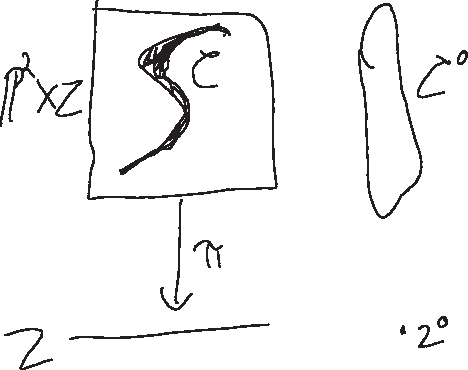
\includegraphics[width=0.5\textwidth]{2011-02-09_Diagram_001}\end{center}
        
        The \emph{fiber} $\mathcal C^0 = \pi^{-1}(z^0)$ of $\mathcal C$ over a point $z^0\in Z$ is the curve whose equation is the polynomial obtained.
        
        by substituting $z_\nu^0$ for $z_\nu$.  The 3 partial derivatives $F_x$, $F_y$, $F_z$ are polynomials in $x$, $y$, $z$, $\{z_\nu\}$ linear in $z_\nu$ and homogeneous of degree $d - 1$ in $x$, $y$, $z$.  They define some subvariety of $\mathbb P^2\times Z$.  Let $S$ be the variety $\{F_1 = F_2 = F_3 = 0\}$.  Note that $S \subset \mathcal C$ (by Euler).
        
        The fiber $\mathcal C^0$ over a point $z^0$ of $Z$ is smooth if and only if $\mathcal C^0$ doesn't meet $S$.
        
        We can construct $\Sigma = \pi(S)$ the image of $S$ via a polynomial $\mathbb P^2 \times Z \to Z$.  Later we'll prove that the image of the projection of any Zariski closed subvariety of $\mathbb P^2 \times Z$ to $Z$ is also Zariski closed.
        
        So the set $\Sigma$ is closed in the affine space $Z$.  But $\Sigma$ is not all of $Z$ (because the Fermat curve is smooth).  So $\Sigma \subset Z$ is a proper closed subvariety.  So the set of $z^0$ for which $\mathcal C^0$ is smooth is a Zariski open subset of $\mathbb A^N$.
      \end{proof}
\end{notessection}


\begin{notessection}{2}{11}{2011}
  Last time, we gave a proof that almost every plane curve of degree $d$ is smooth parameter space $\mathbb A^N$ : $N = \binom{d+2}{2}$.
  
  Another proof, continuing from the middle of the last one:
  \begin{proof}
    The dimension of $S$ (as defined last time) is $N + 2 - 3 = N - 1$ (the three from $F_x = F_y = F_z = 0$).  So $\pi(S)$ is at most $N - 1$ dimensional, and so it's $\overline{\pi(S)}$.  But $\dim Z = N$, so $\overline{\pi(S)} \ne Z$.
  \end{proof}
  
  \paragraph{Some words about topology} $\mathbb A^N= \mathbb C^N$ is a complex variety of dimension $N$. As a real manifold, it's dimension is $2N$.
  In the complex topology, you can have closed disks, e.g. $|z| \le 1$ (has positive measure).  In the Zariski topology, closed subsets have no measure.  e.g., in $\mathbb C$, the only closed subsets are finite point sets.  In $\mathbb C^2$, $V(ax + by + c)$ has no measure (it's a complex plane (dimension 1)).
  
  \begin{prop*}
    A smooth curve $C$ of degree 3 in $\mathbb P^2$ contains exactly 9 flex points.
  \end{prop*}
  \begin{proof}
    Let $f$ be a cubic defining $C$.  The second partial derivatives of $f$ are linear, so the determinant of the Hessian is a cubic polynomial which defines the Hessian curve $H$.
    \begin{thm*}[B\'ezout's theorem]
      A curve of degree $m$ in $\mathbb{P}^2$ intersects a curve of degree $n$ in exactly $mn$ points.
    \end{thm*}
    By this theorem (not yet proved), the two cubics $C$ and $H$ intersect in 9 points.  One can show that the multiplicities are one, and that $C$ and $H$ don't have a factor in common.  Thus, we get exactly 9 flexes.
  \end{proof}
  
  \begin{eg*}
    $y^2 = x^3 - x$ \\
    homogenization gives $y^2z = x^3 - xz^2$ \\
    Then \fbox{$f = x^3 - xz^2 - y^2z$}. \\
    The Hessian matrix is $$\begin{bmatrix} 6x & 0 & -2z \\ 0 & -2z & -2y \\ -2z & -2y & -2x \end{bmatrix}$$
    Then $H(f) = 8(3zx^2 - 3y^2x + z^3)$.  \\
    The flexes: You can eliminate $z$ from $f = H(f) = 0$.  Then you get a homogeneous polynomial in $x$ and $y$.  You can solve for $x / y$, let $y$ be 1, and then plug back in and solve for $z$.  In this example, we get that one of the flex points is at $(x:y:z) = (0:1:0)$.
  \end{eg*}
  
  \subsection*{Genus and Euler characteristic}
    Goal: Want to understand the topological structure of smooth plane curves.
    
    It's useful to put them in a family.  Notation as above.  Let $U = Z  - \Sigma = Z - \pi(S)$.  This is the parameter space for smooth plane curves of degree $d$.  The smooth plane curves are the fibers of the projection $\mathcal C\subset \mathbb P^2 \times U$ to $U$.  
    
    \begin{prop*}
      All the smooth curves of degree $d$ are homeomorphic to each other (as real manifolds of dimension 2).
    \end{prop*}
    \begin{proof}
      The problem set shows that $U$ is path-connected (in the complex topology).  Connect the two points in $U$ (which correspond to curves in $\mathbb P^2 \times U$) by a path.
      
      \begin{center}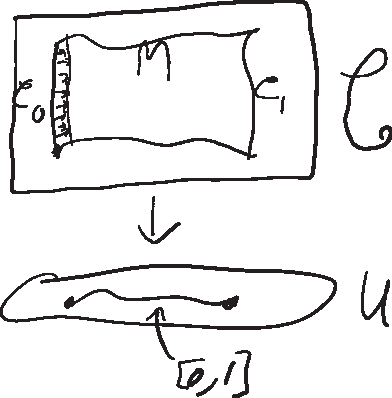
\includegraphics[width=0.5\textwidth]{2011-02-11_Diagram_001}\end{center}
      
      We have a function $f: M \to [0, 1]$.  Define a diffeomorphism by taking the gradient of $f$, and look at the gradient flow.  This tells us how to identify the fibers.
    \end{proof}
    
    \begin{cor*}
      Smooth plane curves are orientable, connected surfaces.
    \end{cor*}
    \begin{proof}
      Orientability is simple.  To orient a smooth surface, we must give a continuously varying orientation to the tangent planes.  But tangent plane is a $\mathbb C$-vector space (of dimension one, $\sum f_i(p) v_i = U$).  So multiplying any tangent vector by $i$ defines a counterclockwise rotation by $90^\circ$, which orients the tangent plane.
      
      We'll do connected next time.
    \end{proof}
  
\end{notessection}

\begin{notessection}{2}{14}{2011}
  \subsection{Plane curves}
    monomials $m_1, \ldots, m_N$, coefficients $z_1,\ldots, z_N$
    \begin{align*}
      Z & = \text{the space of all homogeneous polynomials of degree $d$ in $x$, $y$, and $z$} \\
        & = \text{affine space with coordinates $z_\nu$}
    \end{align*}
    (We have $f(x, y, z) = z_1x^d + z_2 x^{d-1} + \cdots$)
    
    $U = $ open subset in $Z$ corresponding to smooth plane curves
    
    $\mathcal C \subset \mathbb P^2 \times Z$
    
    $$
    \xymatrix{
    \mathcal C \ar[drr] & \subset & \mathbb P^2 \times Z \ar[d] && \mathcal C|_U = \mathcal C_U \ar[drr] & \subset & \mathbb P^2 \times U \ar[d] \\
                       &         &  Z                           && && U
    }
    $$
    
    \begin{prop*}
      Smooth plane curves are orientable and connected surfaces, and compact.
    \end{prop*}
    \begin{proof}
      Oreintability was done last time.
      
      To check connectedness, we just need to check one smooth curve of degree $d$ is connected.  $\mathcal C : \{ x^d + y^d - z^d = 0 \}$.
      
      Look at the line $y = z$.  On $U_2$, taking $z = 1$ we have $x^d + y^d = 1$.  Since $y = z$, $y = 1$, and then $x^d = 0$.  Since this is a root of order $d$, $C$ meets this line in only one point.  This means that it's connected. (WHY?)
    \end{proof}
    
    Given a connected, orientable, compact surface, it's topologically characterized by $g = \text{the genus} = \text{the \# of holes}$.
    
    \begin{defn*}
      The \emph{Euler characteristic} of $C$ is $2 - 2g$.
    \end{defn*}
    
    The Euler characteristic can be computed used an arbitrary triangulation, and then $E = \text{\# vertices} - \text{\# edges} + \text{\# faces}$.
    
    A sphere is, topologically, a tetrahedron, we have that the Euler characteristic is $4 - 6 + 4 = 2$.  We can do a similar thing for a torus.
    
    What is the Euler characteristic and genus of a smooth plane curve of degree $d$?
    
    Let's represent a smooth plane curve as a branched cover of $\mathbb P^1$.
    
    \begin{enumerate}[{Method }I]
      \item Start with the Fermat curve, and do an explicit calculation.  $C: \{x^d + y^d - z^d = 0\}$ \\
        Taking $z = 1$, $U_2 \simeq \mathbb A^2 \simeq \mathbb C^2$.  Then we have $x^d + y^d = 1$.  Drop $y$ by projection.
        Fix a value $x_0$ for $x$.  Then the line $y = x_0$ intersects the curve in $\le d$ points.
        Typically, we get $d$ values for $y$.
        \begin{enumerate}[{Case }I]
          \item $x_0^d \ne 1$.  Solve $y^d = 1 - x_0^d$.  There are $d$ solution s (if $y$ is a solution, then so is $yr^{2 \pi i j / d}$ for $0 \le j \le d$)
          \item $x_0^d = 1$.  Solve $y^d = 0$.  The only solution is $y = 0$. Now we look at $x_0$.  Triangulate $\mathbb P^1$, which is a sphere, as follows.  There are $d$ values for $x_0$, $x_i^d = 1$, $x_i = e^{2\pi i j / d}$.  
      \begin{center}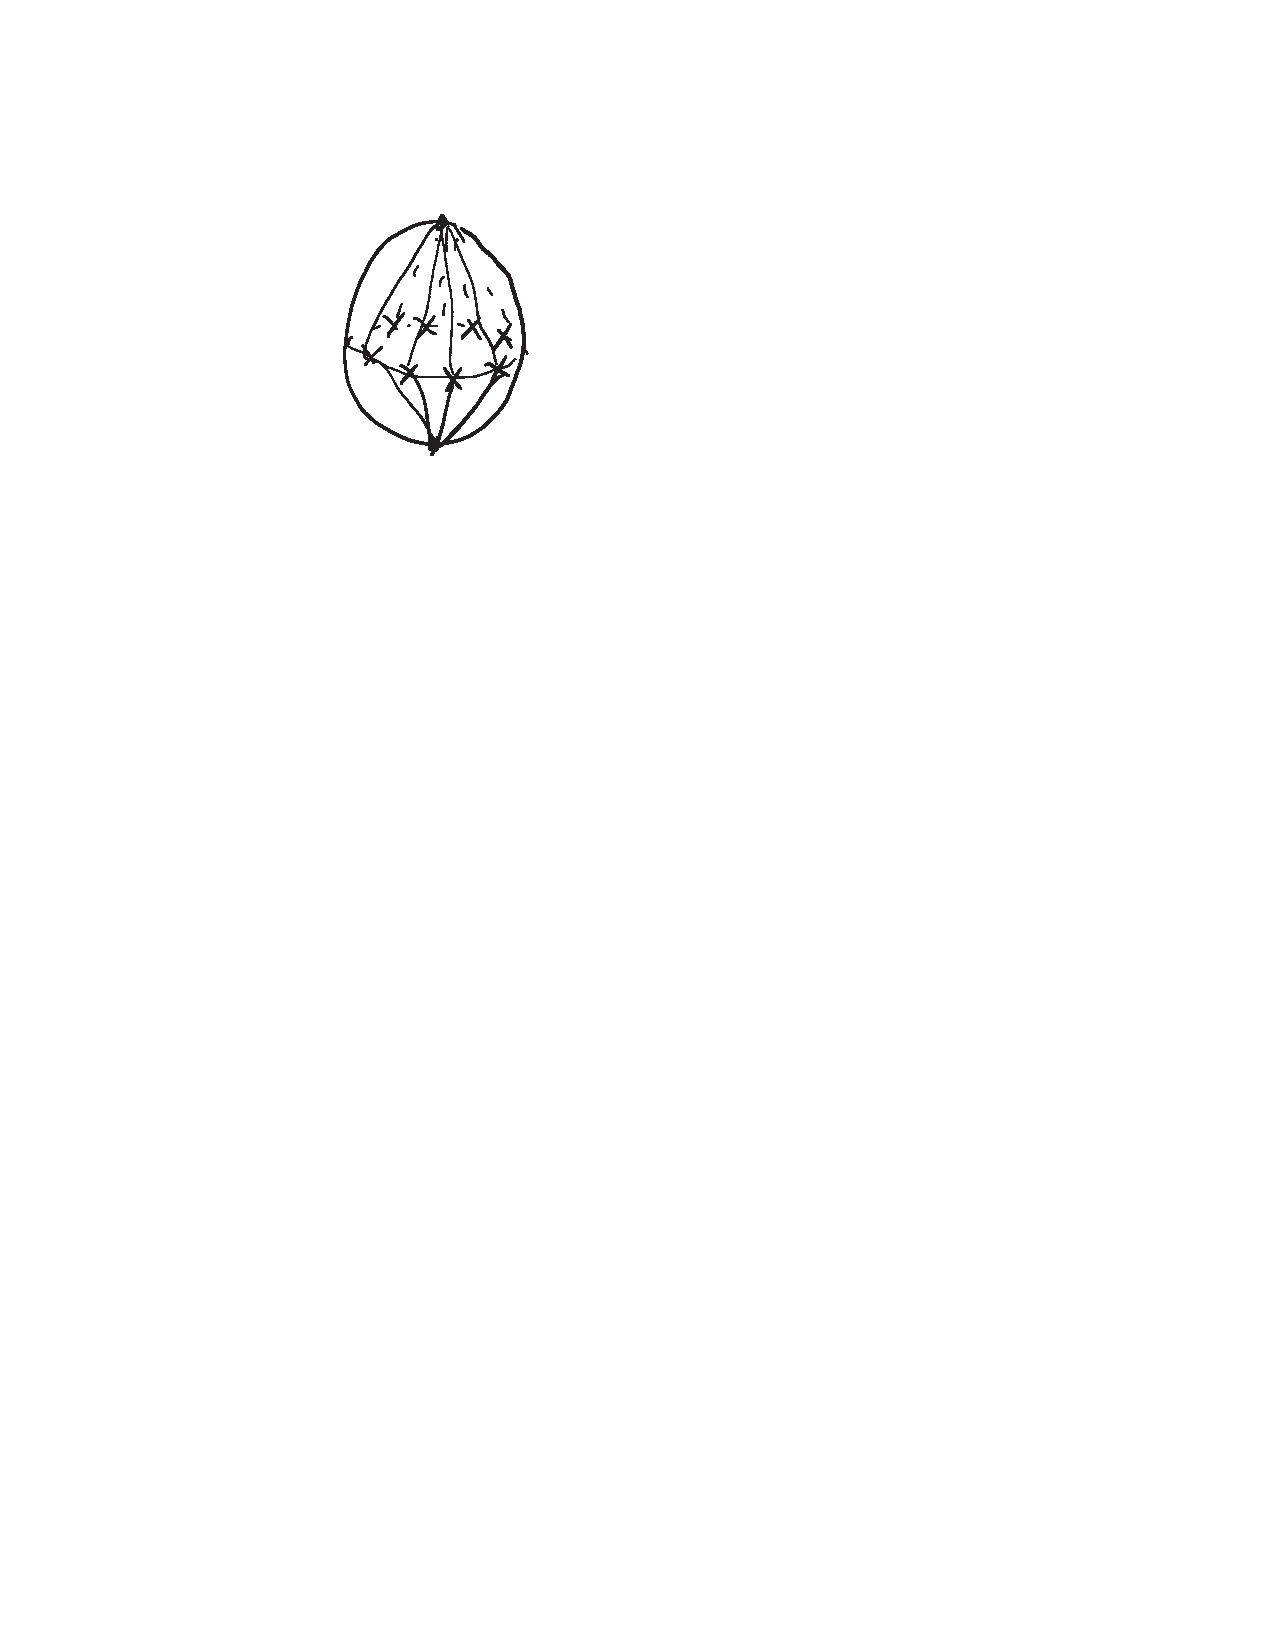
\includegraphics[width=0.3\textwidth]{2011-02-14_Diagram_001}\end{center}
          These points distribute themselves along the equator of $\mathbb P^1$.  Adding points at the poles, there are $2 + d$ vertices, $d + d + d = 3d$ edges, and $2d$ faces, which gives us 2. This is what happens ``downstairs'' (in the projected curve onto $X = \mathbb P^1$).\\
          Upstairs, there is an induced triangulation:
          \begin{itemize}
            \item vertices: $d + d + d = 3d$
            \item edges: $3d^2$
            \item faces: $2d^2$
          \end{itemize}
          Then the Euler characteristic is $E = 3d- 3d^2 + 2d^2 = 3d - d^2 = d(3 - d)$.  Then $g = \frac12(d - 1)(d - 2)$.
        \end{enumerate}
      \item Let $C$ be a smooth curve of degree $d$.  Assume the coefficient of $z^d$ is not zero.  Divide by that coefficient, giving $f(x, y, z) = z^d - a_1(x, y) z^{d-1} + \cdots \pm a_d(x, y)$.  Homogenous polynomial $\implies$ $a_i(x, y)$ is degree $i$ in $x$ and $y$.  Then drop $z$ by projection onto $\mathbb P^1(x, y)$.
        
        Fix $(x_0, y_0)$.  View $z^d - a_1(x_0, y_0) z^{d-1} + \cdots \pm a_d(x_0, y_0) = 0$ as a polynomial of degree $d$ in $z$.  Typically this has $d$ roots, but for some values of $(x, y)$, there are $d-1$ roots.
        
        There is a polynomial $\Delta$, discriminant, degree $d(d - 1)$ in $x$ and $y$.  $\Delta = 0$ iff there are less than $d$ roots.  (The discriminant for a quadratic is $b^2 - 4ac$.  It tells you whether or not the polynomial has double roots.)  (Note, if the discriminant has only simple roots, then the claim above (that there are only $d$ or $d - 1$ roots at any point) is intuitively/geometrically true.)
        
        Triangulate $X = \mathbb P^1$ by putting vertices at these $d(d - 1)$ points.  For $\mathbb P^1$, the Euler characteristic is $2$.  Pulling the triangulation up, the Euler characteristic is approximately $2d$ (everything gets multiplied by $d$).  However, we placed the vertices at the $d(d - 2)$ points where there are $d - 1$ roots.  Then the Euler characteristic is $2d - d(d - 1) = 3d - d^2$.
    \end{enumerate}
\end{notessection}




\begin{notessection}{2}{16}{2011}
  \clearpage
\end{notessection}




\begin{notessection}{2}{18}{2011}
  \clearpage
\end{notessection}




\begin{notessection}{2}{22}{2011}
  \noindent \makebox[\textwidth][c]{\makebox[7.5in][c]{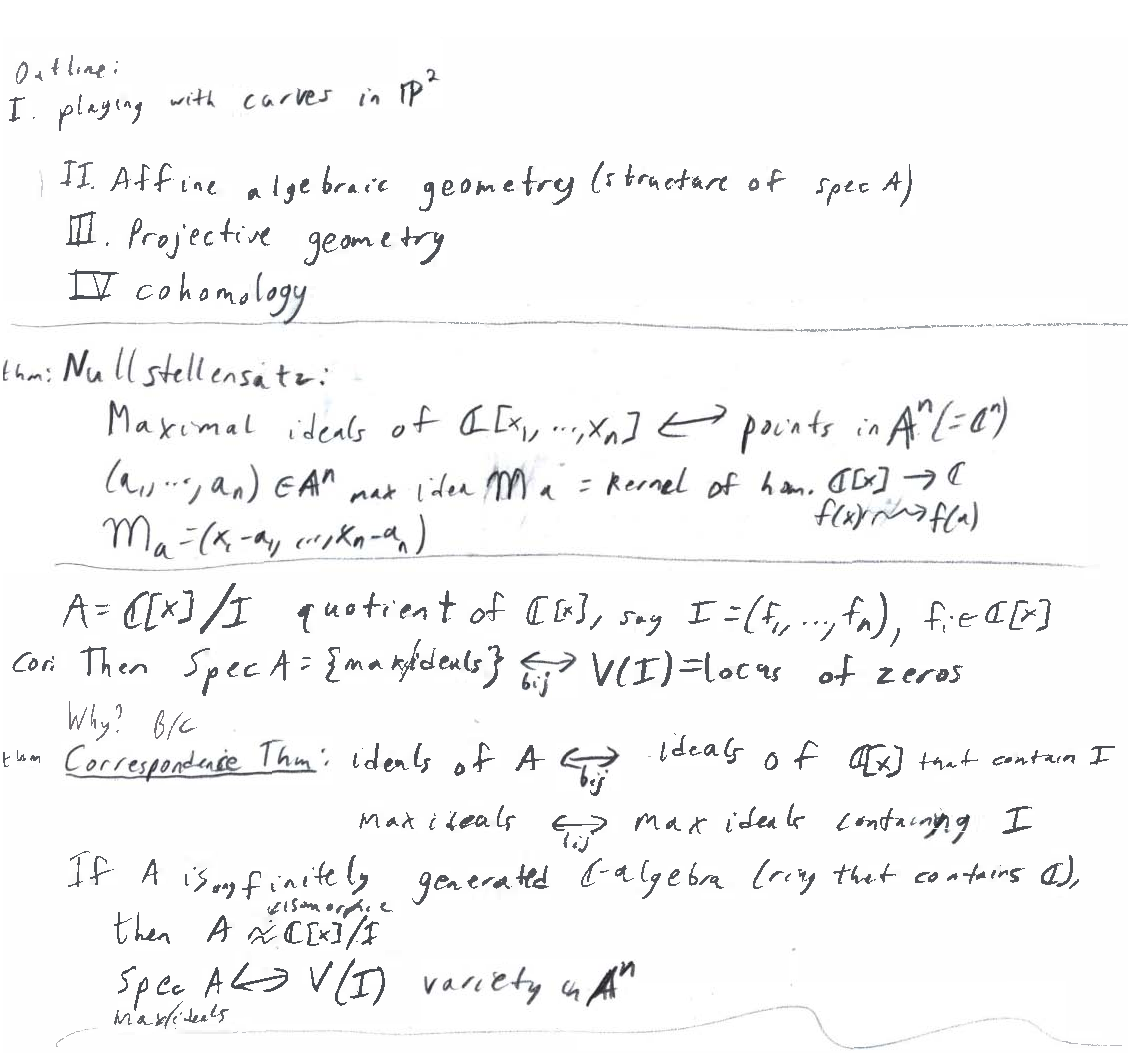
\includegraphics[width=\textwidth]{2011-02-22_Diagram_001}}}
  \clearpage
  \noindent \makebox[\textwidth][c]{\makebox[7.5in][c]{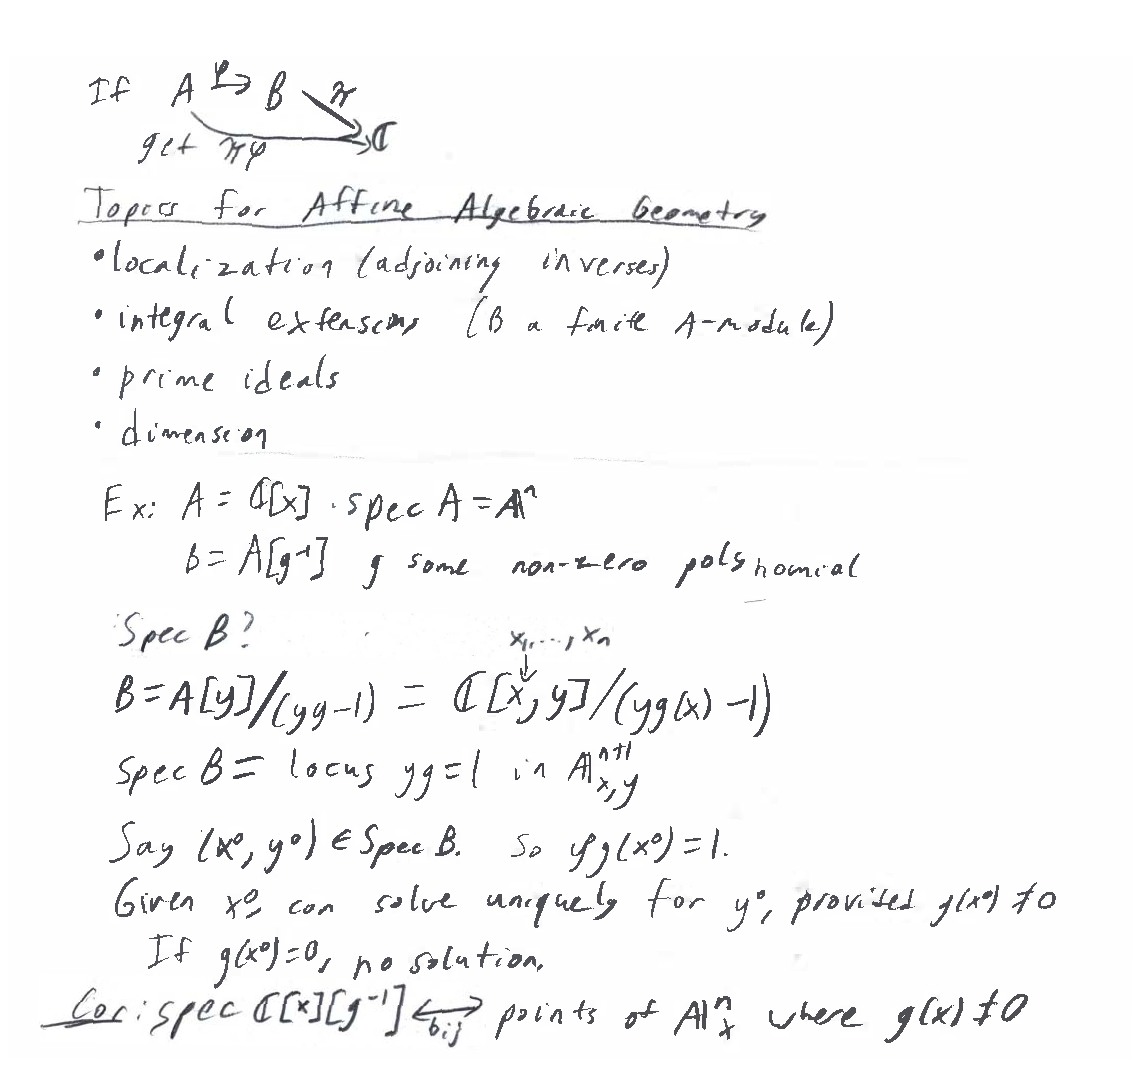
\includegraphics[width=\textwidth]{2011-02-22_Diagram_002}}}
\end{notessection}








\begin{notessection}{2}{23}{2011}
  \subsection*{Hilbert Basis Theorem}
    A ring $A$ is Noetherian if the ideals are finitely generated.
  
    \begin{thm*}[Hilbert Basis Theorem]
      If $R$ is Noetherian, then $R[x]$ is Noetherian
    \end{thm*}
    \begin{cor*}
      $\mathbb C[x_1,\ldots, x_n]$ is Noetherian \\  
      Any finite-type (finitely generated as an algebra (everything is a polynomial in finitely many things)) $\mathbb C$-algebra is Noetherian.  ($A \cong \mathbb C[x] / I$)
    \end{cor*}
  
    \noindent \emph{Equivalent conditions on $A$}:
    \begin{enumerate}
      \item $A$ is noetherian (ideals are finitely generated)
      \item Every infinite increasing family $I_1 \subset I_2 \subset \cdots $ of ideals becomes constant eventually
      \item[] ($I_1 < I_2 < \cdots$ chain is finite)
      \item Every non-empty set $S$ of ideals contains maximal elements ($\exists I \in S$ such that $I \not\subset J$ for any $J \in S$, $J \ne I$)
    \end{enumerate}
    \begin{cor*}
      If $A$ is noetherian,$I$ is an ideal of $A$,  and $I < A$, then $I$ is contained in a maximal ideal.  (The maximal ideal is a maximum element in the set of ideals $< A$.)
    \end{cor*}
    \begin{cor*}
      If $A$ contains no maximal ideal, then $A$ is the zero ring.
      
      $\spec A \ne \emptyset \iff A = \{0\}$
    \end{cor*}
    
    Adjoining inverses to $A = \mathbb C[x]$ ($x = x_1, \ldots, x_n$), $B = A[g^{-1}] = \mathbb C[x, y] / (y g - 1)$.  \\
    Then $\spec A = \mathbb A^n$, and $\spec B \approx \mathbb A^n - V(g)$.
    
    \begin{thm*}[Strong Nullstellensatz]
      Let $I$ be an ideal of $\mathbb C[x]$, $g\in \mathbb C[x]$.  Suppose $g$ vanishes identically on $V(I)$.  Then $g^N \in I$ for some $N \gg 0$.
    \end{thm*}
    \begin{proof}
      \emph{Idea}: Find a ring with no maximal ideal.  It is therefore the zero ring.  Play with this fact.
      
      Say $I = (f_1, \ldots, f_r)$, $f_i \in \mathbb C[x]$ ($x = x_1, \ldots, x_n$).  Let's inspect the locus of zeros in $\mathbb A^{n+1}_{x,y}$, $V = V(f_1, \ldots, f_r; yg - 1)$.
      
      If $(x^0, y^0) \in V$, then $x^0 \in V(I) = V(f_1, \ldots, f_r) \subset \mathbb A^n_x$.  Therefore $g(x^0) = 0$ (by hypothesis).  Then there is no $y^0$ such that $y^0 g(x_0) = 1$.
      
      Therefore, $V = \emptyset$.
      
      We also have that $V = \spec \mathbb C[x, y] / (f_1, \ldots, f_r, yg - 1)$.  Then $\mathbb C[x, y] / (f, yg - 1) = \{0\}$.  Therefore, $(g, yg - 1)$ is the unit ideal in $\mathbb C[x, y]$.  This means that we can write 1 as a polynomial combination of $f$ and $yg - 1$.  Say
      $$1 = p_1(x, y)f_1(x) + \cdots + f_r(x, y) f_r(x) + q(x, y) (y g - 1).$$
      Now work in the ring $B = \mathbb C[x][g^{-1}] = \mathbb C[x, y] / (y g - 1)$.  In $B$ $yg - 1 = 0$ and $y = g^{-1}$.  Then
      $$1 = p_1(x, g^{-1}) f_1(x) + \cdots + p_r(x, g^{-1}) f_r(x) + 0.$$
      Multiply by $g^N$ to clear denominators.  Then, since $g = g(x)$,
      $$g^N = \tilde p_1(x) f_1(x) + \cdots + \tilde p_r(x) f_r(x).$$
      Therefore, $g^N \in I$.
    \end{proof}
    
    \textsc{Note}: If $I \subset J$ are ideals in $\mathbb C[x]$, then $V(I) \supseteq V(J)$.  But $V(x_1) = V(x_1^2)$.
    
    Let $I$ be an ideal.  Then $\operatorname{rad}I = \text{radical of }I = \mathset[g]{g^n \in I,\text{ some }n > 0}$.
    
    \begin{thm*}
      $$V(I) \supset V(J) \iff I \subset \operatorname{rad}J$$
      $$V(I) = V(J) \iff \operatorname{rad}I = \operatorname{rad} J$$
    \end{thm*}
    \begin{proof}
      Say $V(I) \supset V(J)$.  Take $g\in I$.  Then $g = 0$ on $V(J)$.  Then $g^N \in J$ for some $N$ by the strong Nullstellensatz, and so $g \in \operatorname{rad} J$.
      
      The other direction is left as an exercise.
    \end{proof}
    
    \begin{defn*}
      Let $X$ be a topological space.  Then a closed subset $C$ is \emph{irreducible} if you can't write $C = C_1 \cup C_2$ where $C_i$ closed, $C_i < C$.
    \end{defn*}
    
    $A$ a finite type algebra is noetherian, satisfies the ascending chain condition on ideals.  Then $\spec A$ has the descending chain condition on ideals.  
    
    \noindent \emph{Prime ideals}: Given a polynomial ring $R$: (equivalent conditions)
    \begin{itemize}
      \item $R / P$ is a domain
      \item $P < R$, $ab\in P \implies a \in P$ or $b\in P$
      \item $A$, $B$ ideals of $R$, $AB \subset P \implies A \subset P$ or $B \subset P$.  (Recall that the product ideal $AB  = \mathset[\text{finite sums }\sum a_i b_i]{a_i\in A, b_i\in B}$.)
    \end{itemize}
    \begin{proof}
      (2) $\implies$ (3) \\
      Say $AB \subset P$, but $A \subset P$. \\
      $\exists a\in A$, $a\notin P$. \\
      $AB \subset P \implies B \subset P$ \\
      $\forall b\in B$, $ab\in P$, $\therefore b\in P$, so $B\subset P$.
    \end{proof}
    
\end{notessection}






\begin{notessection}{2}{25}{2011}
   \noindent \emph{Recall}: \\
  If $I$ is an ideal of $A$, then $\operatorname{rad}I = \mathset[x \in A]{x^n \in I\text{, some }n > 0}$ \\
  $V(I) = V(\operatorname{rad}I)$ \\
  $V(I) \supset V(J) \iff I \subset \operatorname{rad}J$
  
  irreducible closed set $C$: $C \ne C_1 \cup C_2$, $C_i < C$.
  
  \begin{prop*}
    $I$ an ideal, $V(I)$ irreducible $iff$ $\rad I$ is prime ideal
  \end{prop*}
  
  \begin{thm*}
    Let $A$ be a finite-type noetherian ring, $I$ an ideal.  Then $\rad I$ is the intersection of a finite number of prime ideals $\rad I = P_1 \cap \cdots \cap P_k$.  Then we can organize $P_i \not\subset P_j$ for $i \ne j$.  Then we have that $V(I) = V(P_1) \cup \cdots \cup V(P_k)$; $V(I)$ is a finite union of irreducible closed sets.
  \end{thm*}
  \noindent $\spec A = \{\text{maximal ideals}\}$ \\
  $V(I) = \{\mathfrak M\text{ that contains }I\}$ \\

  $I$ an ideal.  Then $\bar A = A / I$.
  \begin{align*}
    A & \to \bar A \\
    I & \leadsto (\bar 0) \\
    \rad I & \phantom{\to} \rad(\bar 0) \\
    & = \text{\emph{nilradical}} \\
    & = \mathset[x]{x^n = 0}
  \end{align*}
  The following are equivalent:
  \begin{itemize}
    \item $\rad I = P_1 \cap \cdots \cap P_k$
    \item $\rad(\bar 0) = \bar P_1 \cap \cdots \cap \bar P_k$
    \item[] (in $\bar A$)\quad also prime ideals
  \end{itemize}
  \begin{proof}
    Suppose the theorem is false for some $A$ and some $I$.  Let $S = \{\text{ideals }J\text{ of }A\text{ such that }\rad J$ is not a finite intersection of prime ideals$\}$.  By hypothesis, $S \ne \emptyset$.  Then there exists a maximal element $I$ in $S$.  Then $\rad I$ not a finite intersection of prime ideals, but every larger ideal is a finite intersection of prime ideals.  
  
  \noindent \emph{Note}:
  \begin{itemize}
    \item $I = \rad I$
    \item $I$ is not a prime ideal
  \end{itemize}
  Then there exist ideals $K$, $L$, $K\not\subset I$, $L \not\subset I$, but $KL \subset I$.  Replace $K$ by $K + I$, $L$ by $L + I$.  Then we have
  $$(K + I)(L + I) \subset KL + KI + IL + II \subset I.$$
  (so it's ok to do these replacements).

  Now $K, L > I$.  Replace $K$ and $L$ with their radicals.
  $$(\rad K)(\rad L) \subset \rad(KL) \subset \rad I = I$$
  (so it's ok to these replacements.)

  We have
  \begin{align*}
    \rad K & = P_1 \cap \cdots \cap P_r \\
    \rad L & = Q_1 \cap \cdots \cap Q_s
  \end{align*}
  \ldots

  We made a mistake somewhere.  (Supposed to replace $I$ by a zero ideal?)  The version on the web is probably correct.  Let's skip this for now.

  \end{proof}

  \subsection*{Finite Group Action}
    Let $B$ be a finite type domain, $G$ the finite group of automorphisms of $B$.  Let $A = B^G$.
    
    \begin{thm*}
      \begin{itemize}
        \item $A$ is a finite type domain
        \item $G$ operates on $\spec B = Y$
        \item $Y$ maps to $\spec A = X$.  $Y \to X$ is surjective, and the fibers are the $G$-orbits in $Y$
      \end{itemize}
    \end{thm*}
    \begin{example*}
      $B = \mathbb C[x, y]$, $\sigma (x) = -x$, $\sigma(y) = -y$.  Then $\langle \sigma \rangle$ is a group of order 2.

      The invariant functions are $u = x^2$, $v = y^2$, and $w = xy$.  It's not hard to see that every invariant function can be written as some combination of these.

      $A = B^G = \mathbb C[u, v, w] / (w^2 - uv)$

      Then $\spec A = X = \text{locus of }w^2 = uv$ in $\mathbb A^3_{u,v,w}$.  This is a double cone in 3-space.
    \end{example*}
    \begin{proof}
      \noindent \emph{$A$ finite type domain}: \par
      Take $\beta \in B$, orbit $\{b_1 = \beta, \ldots, b_r\}$.  Let $p(x) = (x - b_1)\cdots (x - b_r) = x^r - s_1(b) x^{r-1} + \cdots \pm s_r(b)$.  We have that $\beta$ is a root of $p(x)$.  Since the $s_i(b)$ are symmetric functions, $s_i(b) \in B^G = A$.

      Since $B$ is a finite type domain, say $B$ is generated as an algebra by $\beta_1, \ldots, \beta_m$.  Then each $\beta_i$ is a root of the polynomial, coefficients in $A$.

      Let $A_0 = \mathbb C$-algebra generated by these roots.  Then $A_0$ is a finite-type domain contained in $B$.  Every element in $B$ is a polynomial in $\beta_1, \ldots, \beta_m$.

      If a polynomial with $\beta_i$ as a root has degree $d_i$, then we only need monomials in $\beta_i$ with degree $\le d_i$.  There are only a finite number of monomials in $\beta_i$ of degree $\le d_i$.  Then $B$ is spanned as an $A_0$-module by these monomials.  Thus, $B$ is a finite $A_0$-module.

      $A_0 \subset A \subset B$.  Since $A_0$ is a finite-type domain, $A_0$ is noetherian.  $B$ is a finite-type $A_0$-module.  $A$ is a submodule.  Therefore, $A$ is a finite-type $A_0$ module.  Thus, $A$ is a finite-type algebra.
    \end{proof}
\end{notessection}









\begin{notessection}{2}{28}{2011}
  \begin{itemize}
    \item[] $B$ finite type, $G$ operator(?)
    \item[] $A = B^G$
    \item[] Showed $A$ finite type
    \item[] $Y = \spec B$
    \item[] $X = \spec A$
    \item[] $X \leftrightarrow \{G\text{ orbits in }Y\}$
    \item[] $G \times B \to B$
    \item[] $\sigma, b \leadsto \sigma(b)$
    \item[] (left) $\sigma \tau(b)$: first $\tau$, then $\sigma$
    \item[] Then $G$ operates on the \emph{right} on $Y$.
    \item[] $q\in Y$, $\sigma$ sends $q\to q^\sigma$
    \item[] $q^{\sigma\tau}$: first $\sigma$, then $\tau$
  \end{itemize}
  View
  \begin{align*}
    y & \leftrightarrow \{\text{homomorphisms }B \to \mathbb C\} \\
    q & \leftrightarrow \pi_q: B \to \mathbb C \\
    & \leftrightarrow \{\text{max ideals of }B\} \\
    q & \leftrightarrow m_q
  \end{align*}
  Operation on $Y$:
  $$
  \xymatrix{
    B \ar[r]^\sigma \ar[dr]_{\pi \circ \sigma} & B \ar[d]^\pi \\
                                               & \mathbb C
  }
  $$

  $\pi_q \circ \sigma(b) = \pi_q(\sigma b)$

  Define $q^\sigma = $ that point such that $\pi_{q^\sigma} = \pi_q \circ \sigma$.

  \noindent \emph{Operation on max ideals}: \\
  $\mathfrak M_{q^\sigma} = \sigma^{-1}\mathfrak M_q$ \\
  $Y \to X$? \\
  For any $p\in X$,
  $$
  \xymatrix{
    B \ar[r]^{\pi \circ p} & \mathbb C \\ % fix
    A \ar@{-->}[ur]_{\pi_p}  \ar@{^{(}->}[u]
  }
  $$
  $Y \to X$ sends $q  \leadsto r$ \\
  $$
  \xymatrix{
    B \ar[r]_{\sigma} \ar@/^/[rr]^{\pi} & B \ar[r]_{\pi_q} & \mathbb C \ar@{=}[d] \\
    A \ar@{^{(}->}[u] \ar[r]^{\text{id}} \ar@/_/[rr]_{\pi_p} & A  \ar@{^{(}->}[u] \ar[r]^{\pi_p} & \mathbb C
  }
  $$
  Therefore, $G$-orbits in $Y$ map to points of $X$.

  We want to show that different orbits $\{q_1, \ldots, q_r\} \ne \{q_1', \ldots, q_s'\}$ in $Y$ map to different points $p$, $p'$ in $X$.

  \begin{proof}
    \emph{Plan}: Find an element $a\in A$ such that $a = 0$ on orbit $\{q_i\}$, $\pi_q(a) = 0$, $a \ne 0$ on orbit $\{q'_j\}$.  Then $\pi_{q'_j}(a) \ne 0$.  This would give us that $a\in \mathfrak M_{q_i}$ (same as $\in \mathfrak M_p$) and $a\notin \mathfrak M_{q'_j}$ (same as $\notin \mathfrak M_{p'}$).
  
    In $B$, choose $b\in \mathfrak M_{q_1}$ (then ) such that $b\notin \mathfrak M_{q'_j}$ for all $j = 1, \ldots, s$.  (Note: $b(q) \defeq \pi_q(b)$.)

    \begin{digression}
      Diversion: Suppose $B = \mathbb C[x_1, \ldots, x_n] / (f_1, \ldots, f_k)$.  $b$ represented by the polynomial $p(x_1, \ldots, x_n)$.  $\spec B \approx V(f_1, \ldots, f_k)$ in $\mathbb C^n$.

      $\spec B = (\text{max ideals}) = (\text{homomorphisms }B \to \mathbb C) = (V(I)\text{ if }B = \mathbb C[x] / I)$)
    \end{digression}
    
    We can do this. (Think about choosing (hyper-?)planes that do not pass through finite sets of points.)

    Let $a = \displaystyle \prod_{\sigma\in G} \sigma(b)$.  $a$ is invariant.  $a = 0$ on $q_1$ because $b$ divides $a$ in $B$ (since some $\sigma \in G$ is the identity).  Therefore $a = 0$ on the orbit $(q_1)$.  $a \ne 0$ on $q'_1$.

    $\sigma(b)$ evaluated at $q'_1$ is $\pi_{q'_1}(\sigma b) = \pi_{{q'}_1^\sigma}(b) = b$ evaluated at ${q'}_1^\sigma$.

    Therefore, $a \ne 0$ on the orbit.
  \end{proof}

  \subsection{Localization}
    Note: we always assume that the rings are domains and assume (whenever possible) that they're finite type algebras.

    \begin{defn*}
      A \emph{multiplicative system} $S$ in a domain $A$ is a subset of $A$ satisfying
      \begin{itemize}
        \item $1 \in S$
        \item $0 \notin S$
        \item if $s, t\in S$, then $st \in S$
      \end{itemize}
    \end{defn*}
    \begin{defn*}
      The elements of $S$ serve as denominators in the \emph{ring of fractions}
      $$A_S \defeq \left.\mathset[ \frac{a}{s} ]{s\in S, a\in A}\right/\sim$$
      where $\frac{a}{s} \sim \frac{b}{t}$ if $at = bs$
    \end{defn*}
    \begin{align*}
      A & \hookrightarrow A_S \\
      a & \leadsto a / 1
    \end{align*}
    \begin{example*}
      $S = \{1, s, s^2, \ldots\}$, $s \ne 0$.  $A_S = A[s^{-1}] = A[y] / (sy - 1)$
    \end{example*}
    \begin{example*}
      $S = A - \{0\}$, $A_S = $ fraction field
    \end{example*}
    \begin{example*}
      $P$ a prime ideal of $A$, $S = A - P = \mathset[s]{s\notin P}$.  Then $s\notin P$, $t\notin P$ $\implies$ $st\notin P$.  Then $A_S$ is the \emph{localization of $A$ at $P$}.  This is (perversely) denoted $A_P$.
    \end{example*}

    If $A \subset B$ a subring, then we can relate ideals of $A$ and $B$: \\
    \emph{Extended ideal}: $I^e$
    \begin{itemize}
      \item[] $I$ ideal of $A$
      \item[] $IB = $ ideal of $B$ generated by $\{I\}$
      \item[] The elements are $$\sum_{\text{finite}} x_i b_i\qquad,\ x_i\in I,\ b_i\in B$$
    \end{itemize}
    \emph{Contracted ideal}: $J^c$: For $J$ an ideal of $B$, $(J \cap A) = $ ideal of $A$

    \begin{itemize}
      \item[] $(I^e)^c \supset I$
      \item[] $(J^c)^e \subset J$
    \end{itemize}
    
    For $A \subset B = A_S$:
    \begin{itemize}
      \item[] $I^e = IA_s = \mathset[x / s]{x\in I,\ s\in S} / \sim$
    \end{itemize}

    $J^c = J \cap A$.  If $y / s\in J$, then $y\in J \cap A = J^c$.  Therefore, $y / s\in (J^c)^e$.  Thus, $J \subset (J^c)^e$, so $J = (J^c)^e$.

    \begin{cor*}
      If $A$ noetherian, then $A_S$ noetherian
    \end{cor*}
    \begin{proof}
      Take an increasing sequence $J_1 \subset J_2 \subset \cdots$ of ideals in $A_S$.  Let $I_\nu = J_\nu \cap A$.  Then $I_1 \subset I_2 \subset \cdots$.  Since $A$ is noetherian, this is eventually constant.  Therefore $I_\nu^e = (J_\nu^c)^e$ eventually constant.  Thus $A_S$ is noetherian.
    \end{proof}
\end{notessection}










\begin{notessection}{3}{2}{2011}
  \begin{itemize}
    \item[] $S$ a multiplicative system
    \item[] $1\in S$
    \item[] $0\in S$
    \item[] $S_1, S_2\in S \implies S_1S_2\in S$.
    \item[] Ring of fractions $A_S$ localized ring
    \item[] $A \hookrightarrow A_S$
    \item[] $(J^c)^e = J$
    \item[] $(A \cap J)A_S$
  \end{itemize}
  
  Localizing prime ideal (s...?)
  
  $I$ ideal of $A$, $I \cap S \ne \emptyset\ \implies I^e = $ unit ideal of $A_S$
  \begin{prop*}
    $P$ prime ideal of $A$.  $P \cap S \ne \emptyset$.  Then
    \begin{itemize}
      \item $(P^e)^c = P$
      \item $P^e$ ( $ = P_S$) is a prime ideal of $A_S$
      \item[] $P^e = PA_S = \mathset[s^{-1} x]{x\in P}$
    \end{itemize}
  \end{prop*}
  \begin{proof}
    For any ideal $P$, $(P^e)^c \supset P$.
    
    We want to show $\subset$.  Let $z\in (P^e)^c$.  Then $z = s^{-1}x$ for some $x\in P$, and $z\in A$.  Then $sz = ss^{-1}x = x \in P$.  Since $P$ is prime, and $s\notin P$, $z\in P$, and so $(P^e)^c \subset P$.
    
    Now we show that $P^e$ is prime: \\
    We have that $z_1z_2 \in P^e$ for $z_i \in A_S$.  Then $z_1 = s_1^{-1}a_1$, $z_2 = s^{-1}_2 a_2$.  Then $z_1z_2 = (s_1s_2)^{-1}(a_1a_2) \in P^e$.  Therefore $(s_1s_2)(z_1z_2) = a_1a_2 \in P^e$.  Since $a_1a_2 \in A$, this is also in $(P^e)^c = P$.  Since $a_1a_2 \in P$ and $P$ prime, either $a_1\in P$ or $a_2\in P$, $s_1^{-1} a_1 \in P^e$ or $s_2^{-1}a_2\in P^e$.\footnote{Sorry if this proof is unclear.  I was trailing behind Prof. Artin, and so wasn't understanding the proof well.}
  \end{proof}
  
  $$P\spec A_S \longleftrightarrow \text{subset of }P\spec A = \mathset[P]{P\cap S\ne \emptyset}$$
  
  Back to the case where $P$ is a prime ideal of $A$ and $S = A - P = \mathset[s\in A]{s\notin P}$. \\
  Write $A_P$ for $A_S$.  If $I$ is an ideal of $A$, $I_P = I_S$ extended ideal.
  
  \begin{prop*}
    $P_P$ is a maximal ideal of $A_P$ and it is the only maximal ideal of $A_P$.
  \end{prop*}
  \begin{lem*}
    For a ring $R$, the following are equivalent:
    \begin{enumerate}[(1)]
      \item $R$ has a unique maximal ideal $\mathfrak M$
      \item The elements of $R$ that are not invertible form an ideal
    \end{enumerate}
  \end{lem*}
  \begin{proof}
    \begin{itemize}
      \item[$(2)\implies (1)$] Suppose that the non-units form an ideal $I$.  Then $R / I$ is a field because every element is the residue of a unit, and therefore invertible.  Thus $I$ is a maximal ideal.  Since any other element is a unit, we cannot include any other element without turning the ideal into the entire ring.  Thus, this is maximal.
      \item[$(1) \implies (2)$]  Suppose there exists a unique maximal ideal $\mathfrak M$.  Let $u\in R$.  Then $(u) = R$ if and only if $u$ is a unit.  If $u$ is not a unit, then $(u) < R$, and so $(u) \subset$ some maximal ideal.\footnote{If $R$ is not noetherian, this requires Zorn's Lemma/The Axiom of Choice.}  Then $(u) \subset \mathfrak M$.  Then $\mathfrak M$ contains all the non-invertible elements, and so the non-invertible elements of $R$ form an ideal (in particular $\mathfrak M$).
    \end{itemize}
  \end{proof}
  \begin{proof}[Proposition above]
    \noindent $s^{-1}a \in A_P$, $s\notin P$. \\
    If $a\in P$, then $s^{-1}a\in P_P$.  If $a\notin P$, then $s^{-1}a$ is invertible, and so $a^{-1}s \in A_S$.
  \end{proof}
  \begin{defn*}
    A (noetherian) ring $R$ is \emph{local} if it has a unique maximal ideal $\mathfrak M$.  (Note that $R / \mathfrak M$ is a field.)
  \end{defn*}
  \begin{example*}
    $A = \mathbb C[x, y]$.  The prime ideals are
    \begin{itemize}
      \item $(0)$
      \item $(f(x, y))$ for $f$ irreducible
      \item maximal ideal $\mathfrak M_{(a, b)} = (x - a, y - b) \longleftrightarrow (a, b) \in \mathbb C^2$
    \end{itemize}
    \begin{itemize}
      \item[] $A_{(0)}$: fraction field $\mathbb C(x, y)$ of $\mathbb C[x, y]$
      \item[] $A_{\mathfrak M_{(a, b)}}$: a local ring.  The prime ideals $\pspec A_{\mathfrak M} = \mathset[P]{P\cap S\ne \emptyset} = \mathset[P]{P\subset \mathfrak M} = \begin{cases} (0) & \\ P = (f)\,|\,f(a, b) = 0 & \\ \mathfrak M_{(a, b)} & \end{cases}$
    \end{itemize}
  \end{example*}
  \begin{lem*}
    %\begin{itemize}
      %\item
    Suppose $I$ is an ideal of the ring $A$ and $M$ is a finite $A$-module such that $M = I M$.  Then there exists a $z\in I$ such that $(1 - z)M = 0$.
  \end{lem*}
  \begin{proof}
    Say $(x_1, \ldots, x_r$ generate $M$.  We can write $x_i$ as a combination of $\{x_1, \ldots, x_r\}$ with coefficients in $I$:
    \begin{align*}
      x_i & = \sum_j p_{ij}x_j & p_{ij}\in I \\
      X  & = PX  & P\text{ matrix }(p_{ij}) \\
      (\mathbb{I} - P)X & = 0  \\
      Q(\mathbb{I} - P) = \delta \mathbb{I}
    \end{align*}
    where $Q$ is the cofactor matrix for $\mathbb{I} - P$ with entries in $A$, and $\delta = \det(\mathbb{I} - P)$.
    \begin{align*}
      Q(\mathbb{I} - P)X & = 0 \\
      \therefore \delta X = 0 \\
      \mathbb{I} - P & = \begin{pmatrix} 1 - p_{11} & \cdots&  \\ & \ddots & \\ && 1 - p_{nn} \end{pmatrix} \\
      \delta & = 1 - z
    \end{align*}
    Since the $p_{ij} \in I$, we have $z\in I$.  Then $(1 - z)X = 0$, so $(1 - z)$ kills $M$.
  \end{proof}
  \begin{lem*}[Nakayama Lemma]
    Let $A$ be a local ring with a maximal ideal $\mathfrak M$, and let $M$ be a finite $A$-module.  If $M = \mathfrak M M$, then $M = 0$.
  \end{lem*}
  \begin{proof}
    Take $z\in \mathfrak M$.  We have a $z$ with $(1 - z)M = 0$.  Since $1 - z \notin \mathfrak M$, $1 - z$ is invertible, and so $M = 0$ (since we can multiply by $(1 - z)^{-1}$).
  \end{proof}
  
\end{notessection}










\begin{notessection}{3}{4}{2011}
  \subsection*{Integral Extensions}
    \noindent $A \subset B$ domains \\
    \begin{defn*}
      $b\in B$ is \emph{integral over $A$} if it's a root of a monic polynomial.\\
      $f(x) = x^n - a_1 x^{n-1} + \cdots \pm a_r$ coefficients in $A$ \\
    \end{defn*}
    \begin{prop*}
      The following are equivalent:
      \begin{enumerate}[(1)]
        \item $b$ is integral over $A$
        \item $A[b]$ is a finite $A$-module
        \item There exists an $A[b]$-module $M$ which:
          \begin{enumerate}[(i)]
            \item is faithful\footnote{A module is faithful if for any $z\in A[b]$, $z\ne 0$, $zM \ne 0$.} as an $A[b]$-module
            \item is a finite $A$-module
          \end{enumerate}
      \end{enumerate}
    \end{prop*}
    \begin{proof} \par\noindent
      \begin{itemize}
        \item[$(1) \implies (2)$] Clear
        \item[$(2) \implies (3)$] Clear
        \item[$(3) \implies (1)$] Take the generators for $M$ as an $A$-module, $(v_1, \ldots, v_n)$.  Then $bv_i = \sum a_{ij} v_j$ for $a_{ij} \in A$.  We can write this as
          $$(b \mathbb{I} - A) V = 0\qquad V = \begin{pmatrix} v_1 \\ \vdots \\ v_n\end{pmatrix}$$
          Let $C$ be the coefficient matrix of $(b \mathbb{I} - A)$.  Then $C(b \mathbb{I} - A) = \det(b\mathbb{I} - A)\mathbb{I}$.  Let $\delta \defeq \det(b\mathbb{I} - A)$.  Then $\delta V = 0$.  Since $M$ is faithful, $\delta = 0$.)  Expanding $\delta$ gives $\delta = b^n - (\tr A)b^{n-1} + \cdots \pm \det A$ is a monic polynomial for $b$.  The coefficients are in $A$, so $A[b]$ is integral.
      \end{itemize}
    \end{proof}
    \begin{prop*}
      Let $A$ be noetherian.  
      \begin{itemize}
        \item If $B$ is generated as an $A$-algebra by elements integral over $A$, then every element of $B$ is integral over $A$.
        \item If $B$ is generated over $A$ by a finite number of integral elements, then $B$ is a finite $A$-module.  (e.g., $B$ integral over $A$ and a finite type $\mathbb C$-algebra.)
      \end{itemize}
    \end{prop*}
    \begin{proof}
      Take $z\in B$.  Then $z \in A[b_1, \ldots, b_k]$ for $b_i$ integral.  $A[b_1, \ldots, b_k]$ is a finite $A$-module.  Therefore $A[z]$ is contained in a finite module, so it itself is finite.
    \end{proof}
    \begin{prop*}[Noether Normalization]
      \flag[I'm still confused by this statement.]{
      Let $K$ be a field, and let $A$ be a finite-type $K$-algebra and a domain.  There exist $y_1, \ldots, y_d\in A$ algebraically independent\footnote{There are no polynomial relations among them.}, and $A$ is a finite module over $K[y_1, \ldots, y_d]$.
      }
    \end{prop*}
    $$
    \xymatrix{
      A & \spec A \ar[d] \\
      \mathbb C[y_1, \ldots, y_d] \ar@{^{(}->}[u] & \mathbb A^d
    }
    $$
    \begin{proof}
      Given $A$ generated by $x_1, \ldots, x_n$ (some finite set).  Independent on $n$.(???)
      If $x_1$, \ldots, $x_n$ dependent, there exists a polynomial relation $f(x_1, \ldots, x_n) = 0$ of degree $d$.  Let $h(x)$ be the degree $d$ part of $f$.  Then $h(0,0,0,\ldots, 1) = $ coefficient of $x_n^d$ in $h$ and in $f$.  If the coefficient of $x_n^d \ne 0$, then $f(x)$ looks like $cx_n^d + g_{n-1}(x_1, \ldots, x_{n-1}^{d-1} + \cdots + g_0(x_1, \ldots, x_{n-1})$.  If $c \ne 0$, this is a monic polynomial of which $x_n$ is a root, and its coefficients are in the ring $K[x_1, \ldots, x_{n-1}]$.  Therefore, $x_n$ is integral over $K[x_1, \ldots, x_{n-1}]$.  By induction, we get a tower of integral extensions.
      
      If $c = 0$, then make a change of variables $x_i \mapsto x_i + u_i x_n$ (for $i < n$), $x_n \mapsto u_n x_n$.  Now the coefficient of $x_n^d$ will be $h(x_1 + u_1x_n, \ldots, x_{n-1} + u_{n-1}x_{n-1}, u_n x_n)|_{x_1 = \cdots = x_{n-1} = 0,\ x_n = 1} = h(u_1, \ldots, u_n)$.  This is non-zero for most choices of $u_i$.\footnote{For fields with finite characteristic, you'll have to make a non-linear change of variables.}
    \end{proof}
    \begin{cor*}[A version of Nullstellensatz]
      Let $K$ be a field, $B$ a finite-type $K$-algebra that is also a field.  Then $B$ is a finite $K$-module.
    \end{cor*}
    \begin{digression}
      It follows, without much trouble, from this that if $K = \mathbb C$, $B = \mathbb C$, too; if $B$ is a finite field extension of $\mathbb C$, then $B = \mathbb C$.
      \begin{proof}
        Take $b\in B$.  $\mathbb C[b]$ is a finite $\mathbb C$-module.  Therefore, $b$ is a root of an irreducible polynomial with coefficients in $\mathbb C$.  Therefore, it is a root of a linear polynomial over $\mathbb C$, so $b\in \mathbb C$.
      \end{proof}
    \end{digression}
    \begin{proof}
      Noether Normalization says $B$ a finite module over polynomial ring $A = K[y_1, \ldots, y_d]$.  If $d = 0$, then we're done.  If $d > 0$, then $y_1\in A, B$, so $\frac{1}{y_1} \in B$.  Thus $B$ is a field.  But $\frac{1}{y_1}$ is not integral over $K[y_1, \ldots, y_d]$.
    \end{proof}
    
    If $A$ is a domain with fraction field $K$, then $A$ is \emph{integrally closed} in $K$ if every element of $K$ which is integral over $A$ is an element of $A$.
    \begin{example*}
      $A = \mathbb C[x, y] / (y^2 - x^3)$.  This is not integrally closed: Let $z = \frac{y}{x}$.  \\
      Then $z^2 = \frac{y^2}{x^2} = \frac{x^3}{x^2} = x$.  \\
      $z^3 = \frac{y^3}{x^3} = \frac{x^3y}{x^3} = y$.  \\
      $z$ is a root of the monic polynomial $z^2 - x$, and of $z^3 - y$.
    \end{example*}
    
    \begin{thm*}
      Let $A$ be a finite-type algebra and a domain, and let $K$ be the fraction field of $A$.  Then the \emph{integral closure} of $A$ in $K$, the set of integral elements, is a finite $A$-module.
    \end{thm*}
    
    \noindent Preview:  \\
    Given an $A$-module $M$, then $M^* \defeq \hom_A (M, A)$ is also an $A$-module.
    
    If $M \subset N$, then $M^* \supset N^*$ (in good situations).
\end{notessection}










\begin{notessection}{3}{7}{2011}

\end{notessection}










\begin{notessection}{3}{9}{2011}
  %\subsection*{Corrections from Last Time}
  \begin{thm*}
    Let $A$ be a finite type algebra and a domain, and let $K$ be the field of fractions.  Then the integral closure of $A$ is a finite extension $L / K$, and is a finite $A$-module.
  \end{thm*}
  \begin{proof}
    Had the trace pairing $L \times L \to K$, $x, y \leadsto tr(xy)$.  It's non-degenerate because:
    
    $y x \ne 0$, put $y = x^{-1}$
    
    $\langle x, y \rangle = t(1) = [L:K]$
    
    Reduce to the case of $A$ integrally closed by Noether Normalization.
    
    $k[y] \subset A$, $A$ a finite $k[y]$-module
    
    $k[y] \subset K \subset L$.
    
    Replace $A$ by $k[y]$.
    
    $\therefore$, we may assume that $A$ is integrally closed.  Then if $\alpha \in L$ is integral over $A$, $tr(\alpha) \in A$.
    
    Therefore, if $B$ is any subring of $L$, and a finite $A$-module, then all elements are integral over $A$.  Therefore, $B\times B \to A$, $x, y \leadsto \langle x, y\rangle = tr(xy)$.
    
    \emph{We want to show} that there is a maximal such $B$.  Then $B$ is the integral closure in $L$.
    
    Start with one, $B_0$, big enough so that it contains a basis for $L / K$.  (We can do this because for any $\gamma\in L$, $\gamma$ is algebraic in $K$; $\gamma^n - a_1 \gamma^{n-1} + \cdots \pm a_n = 0$ with $a_i\in K$.  Since $K$ is the field of fractions, we can clear denominators, getting $d\gamma^n - a_1' \gamma^{n-1} + \cdots \pm a_n' = 0$, with $d, a_i'\in A$.  Then $d\gamma$ is integral over $A$; multiply everything by $d^{n-1}$.)  Denote the basis by $(v_1, \ldots, v_n)$, $v_i\in B_0$, $n = [L:K]$.
    
    Investigate some larger algebra (which is still a finite $A$-module) $B$.  Then $A\subset B_0 \subset B$.
    \begin{align*}
      B \times B & \to A \\
      \beta, v_i & \leadsto b_i \defeq \langle \beta, v_i\rangle\in A \\
      \intertext{map}
      \beta & \leadsto (b_1, \ldots, b_n)\in A^n \\
      B & \stackrel{\Phi}{\to} A^n
    \end{align*}
    This is $A$-linear (homomorphism of $A$-modules)
    
    $\Phi$ is injective: $\Phi(\beta) = 0$ means $\langle \beta, v_i\rangle = 0$ for all $i$.  Since $\{v_i\}$ is a basis for $L / K$, $\langle \beta, y \rangle = 0$ for all $y \in L$.  Thus, $\beta = 0$.
    
    Then we can identify $B$ with $\Phi(B)$ as a submodule of $A^n$.  Since $A$ is noetherian, submodules have the ascending chain condition.
  \end{proof}
  
  (DIGRESSION ABOUT GALOIS GROUPS AND $G$-ORIBTS NOT INCLUDED)
  
  Let $A \subset B$ be a domain, $A$ finite-type and integrally closed, and $B$ a finite $A$-module.
  
  What about prime ideals in $A$ and $B$?
  \begin{itemize}
    \item[] extended ideal of $P\subset A$ is $P^e = PB$ ideal of $B$
    \item[] contracted ideal of $Q\subset B$ is $Q^c = A \cap Q$ ideal of $A$
  \end{itemize}
  
  \begin{fact*}[General Fact]
    If $Q$ is a prime ideal of $B$, then $Q^c$ is a prime ideal of $A$.
    $$
    \xymatrix{
      A \ar@{^{(}->}[rr] \ar[dr]_{\text{kernel $Q^c$}} && B \ar[dl]^{\text{kernel $Q$}} \\
      & B / Q \text{\makebox[0pt][l]{a domain ($Q$ prime)}}
    }
    $$
    The image is a domain, so $Q^c$ is a prime ideal.
  \end{fact*}
  
  Back to the case above,
  $$
  \xymatrix @R=0.5em{
    A \ar@{^{(}->}[r] & B \\
    P' & Q' & \text{we mean }P' = A \cap Q' \\
    P & Q & P = A \cap Q,\quad Q'\supset Q
  }
  $$
  
  \begin{fact}[Lying Over]
    Given $P$ a prime ideal of $A$, there exists a $A$ prime ideal of $B$, with $A \cap Q = P$.  (The map $\pspec B \to \pspec A$ is injective.)
  \end{fact}
  
  \begin{fact}[Going Up]
    Given
    $$
    \xymatrix @R=0.25em{
      A \ar@{^{(}->}[r] & B \\
      P' &  *+[o][F.]{Q'} & \ar[l] \text{exists} \\
      P & Q
    }
    $$
  \end{fact}
  
  \begin{fact}[Going Down]
    If $A$ is integrally closed, then given
    $$
    \xymatrix @R=0.25em{
      A \ar@{^{(}->}[r] & B \\
      P' &  Q' \\
      P & *+[o][F.]{Q} & \ar[l] \text{exists}
    }
    $$
  \end{fact}
  
  \begin{lem*}
    Given 
    $$
    \xymatrix @R=0.25em{
      A \ar@{^{(}->}[r] & B \\
      P' &  Q' \\
      P & Q
    }
    $$
    If $P' = P$, then $Q' = Q$.
  \end{lem*}
  \begin{proof}
    \begin{enumerate}[{Case }1:]
      \item $P = 0$.  We need to show that if $P' = 0$, then $Q' = 0$.  Take $\alpha \in Q' \subset B$.  Then $\alpha$ is integral over $A$ (because it's in $B$?).  We have $\alpha^r - a_1 \alpha^{r-1} + \cdots \pm a_r = 0$.  Since $a_r \in Q'$ and $a_r\in A$, we have $a_r \in P' = \{0\}$.  Thus $a_r = 0$.  If $\alpha \ne 0$, then cancel $\alpha$ from the relation, and repeat until $r = 1$.  Then $\alpha^1 - a_1 = 0$.  Since $a_1 \in A$ and $a_1 \in Q'$, $a_1\in P'$.  Then $a_1 = 0$ and $\alpha = 0$, which is a contradiction.
      \item (general case).  Go to $\bar A = A / P \subset \bar B = B / Q$.  
        $$
        \xymatrix @R=0.25em{
          \bar A \ar@{^{(}->}[r] & \bar B \\
          \bar P' &  \bar Q' \\
          (0) & (0)
        }
        $$
        Then case 1 says that $\bar P' = (0)$ implies that $\bar Q' = (0)$.  Then $\bar P' = (0) \iff P' = P$ and $\bar Q' = (0) \iff Q' = Q$.
    \end{enumerate}
  \end{proof}
  \begin{lem*}
    If $Q$ is a maximal ideal of $B$, then $Q^c = P$ is maximal in $A$.
  \end{lem*}
  \begin{proof}
    $Q$ is maximal in $B$ if and only if $\bar B = B / Q$ is a field.  Then $A / P = \bar A \subset \bar B$ is a field.  Then $\bar B$ is a finite $\bar A$-module.
    \begin{lem*}
      If $A \subset B$ is a field and $B$ is a finite $A$-module, then $A$ is a field.
    \end{lem*}
    \begin{proof}
      Take a non-zero element in $\alpha\in A$ (we want to show that it's invertible).  Then $\alpha$ is invertible in $B$.  Since $B$ is a finite $A$-module, so $u = \alpha^{-1}$ is integral over $A$.  Then $u^r - a_1 u^{r-1} + \cdots \pm a_r = 0$ with $a_i \in A$.  Multiply by $\alpha^{r - 1}$.  Then we get $u - a_1 + a_2 \alpha - \cdots \pm a_r \alpha^r = 0$, with all of these elements of $A$.
    \end{proof}
    (To be finished next time?)
  \end{proof}
\end{notessection}










\begin{notessection}{3}{11}{2011}
  Finite group action on an integrally closed finite-type domain $B$, $A = B^G$, (has the?) invariants
  \begin{itemize}
    \item[] $\max A \leftrightarrow G$-orbit in $\max B$
    \item[] $A$ is finite type and integrally closed
    \item[] $B$ is a finite $A$-module
  \end{itemize}
  \begin{defn*}
    $A$ is \emph{normal} if it's integrally closed in the field of fractions of $A$ (i.e., it's own fraction field).
  \end{defn*}
  \begin{thm*}
    Let $G$ be a finite group that acts on an integrally closed finite-type domain $B$, $A = B^G$.  Then
    \begin{itemize}
      \item $\pspec A \leftrightarrow (\pspec B) / G$
      \item This preserves inclusions.  More formally, If $P\leftrightarrow \text{orbit }\{Q_j\}$ and $P' \leftrightarrow \text{orbit }\{Q'_i\}$, then $P \subset P'$ if and only if $\forall j \exists i$ such that $Q_j \subset Q'_i$. \par\noindent
      We have $Q \leadsto A \cap Q$, $\spec B \to \spec A$
    \end{itemize}
  \end{thm*}
  \begin{lem*}
    Let $Q_1, \ldots, Q_m$; $Q_1', \ldots, Q_n'$ be prime ideals of $B$.  Suppose $Q_j \not\subset \text{any }Q_i'$, $j = 1, \ldots, m$, $i = 1, \ldots, n$.  Then there exists $\alpha \in B$, $\alpha \in Q_1, \ldots, Q_m$, $\alpha \notin Q_1', \ldots, Q_n'$.
  \end{lem*}
  \begin{proof}
    Plan: Solve for a single $Q_j$.  Find $\alpha_j\in Q_j$, $\notin Q_1', \ldots, Q_n'$.  Then the product $(\alpha_1 \cdots \alpha_m$) works; $\alpha_1 \cdots \alpha_m \in Q_i' \implies $ some $\alpha_j \in Q_i'$.  This would be a contradiction.
    
    Take $Q_1 = Q$, $Q_1', \ldots, Q_n'$, $\alpha \in Q$, $\notin Q_i'$.
    
    %Hypothesis: $Q \not\subset Q_i'$; Conclusion: $Q \not\subset \bigcap Q_i'$.
    
    $\alpha = \beta_i\in Q$, $\notin Q_i'$, $i = 1,\ldots$. $\beta_1 \cdots \beta_n\in Q$.
    \ldots (Proof not included)
  \end{proof}
  \begin{proof} (of theorem) \par\noindent
    In $C$:
    $$
    \xymatrix @R=1em{
      B \ar[r]^\sigma & B \\
      A \ar@{^{(}->}[u] \ar[r]^{\text{id}} &  A
    }
    $$
    
    Since $Q$ is a prime ideal of $B$ and $P = A \cap Q$, we have that $\sigma Q$ is a prime ideal of $B$ and $P = A\cap \sigma Q$.  Then an orbit of $Q$ corresponds to one point in $\pspec A$.  By the lying over theorem, $\spec B \to \spec A$ is surjective.  Therefore $(\spec B) / G \to \spec A$ is also surjective.
    
    \emph{Injective}:   $\{Q_1, \ldots, Q_m\}$, $\{Q_1', \ldots, Q_n'\}$ distinct orbits.  $A \cap Q_j = P$, $A \cap Q_i' = P'$, show $P \ne P'$.
    \begin{claim*}
      We can't have $Q_i \subset Q_j'$ for some $i$, $j$ and also $Q_k' \subset Q_\ell$ for some $k$, $\ell$.
    \end{claim*}
    \begin{proof}
      We can renumber, $i = j = 1$.  $Q_k' \subset Q_\ell \implies \sigma Q_k' \subset \sigma Q_\ell$.  We may then assume that $\ell = 1$; since $\sigma$ runs through the whole orbit, we can choose an appropriate $\sigma$.
      
      Then $Q_1 \subset Q_1'$, $Q_k' \subset Q_1$.  Then $Q_k' \subset Q_1 \subset Q_1'$.  Then $Q_k' \subset Q_1'$.  Thus $k = 1$, because $Q_k' = \sigma Q_1'$ for some $\sigma$ (and permutations can't take sets to proper subsets of themselves).  Then $Q_1' \subset Q_1 \subset Q_1'$, so $Q_1 = Q_1'$.  This is a contradiction, since orbits are disjoint.  Thus, we may suppose that $Q_j \not\subset Q_i'$ for any $i$, $j$.
    \end{proof}
    There exists an $\alpha \in Q_1 \cap \cdots \cap Q_m$, $\notin Q_i'$.  Take $\gamma = \prod_\sigma \sigma \alpha $, $\gamma\in Q_j$, $\notin Q_i'$, and $\gamma \in A$.  Thus, $\gamma \in P$, $\notin P'$, so $P \ne P'$.
    
    The proof of the second point is skipped  (See notes that Prof. Artin posted).
  \end{proof}
  
  Let $B$ be a finite $A$-module for a normal $A$.  
    $$
    \xymatrix @R=1em{
      A \ar@{^{(}->}[r] & B \\
      P' \ar@{^{(}->}[u] &  Q' \ar@{^{(}->}[u] \\
      P \ar@{^{(}->}[u] & Q \ar@{^{(}->}[u]
    }
    $$
  $P' = A \cap Q'$, $P = A \cap Q$
  
  \begin{thm*}[Going Up]
    In the diagram above, given $P$, $P'$, $Q$, there exists a $Q'$.
  \end{thm*}
  
  \begin{thm*}[Going Down]
    In the diagram above, given $P$, $P'$, $Q'$, there exists a $Q$.
  \end{thm*}
  \begin{proof}
    Let $K$ be the fraction field of $A$ and $L$ be the fraction field of $B$.
    \begin{enumerate}[{Case }1:]
      \item $L / K$ is Galois, has Galois group $G$(?).  $B$ is normal. \par\noindent
        $\sigma$ acts on $B$: The elements of $B$ are integral of $A$.  If $\beta$ is integral, so is $\sigma \beta$.  Then, since $B$ is normal, $B$ is the integral closure of $A$ in $L$.  Thus, $\sigma \beta \in B$.
        
        $A = B^G$. (We know that $B$ is a finite $B^G$-module.):  $A \subset B^G$ and $A$ is normal.  Since $B$ is integral over $A$, $B^G$ is integral over $A$, so $A = B^G$.
        
        Then the theorem follows from the previous theorem.
      \item (general case): $L / G$ not Galois, and/or $B$ not normal:  Put $L \subset F$ a Galois extension of $K$ with Galois group $G$.  Let $C$ be the integral closure of $A$ in $F$.  This is a finite $A$-module.  Then $G$ operates on $C$.  Then $A = C^G$ (by the same reasoning as in case 1).
      
      $$
      \xymatrix @R=0.25em{
        A \ar@{^{(}->}[r] & B \ar@{^{(}->}[r] & C \\
        P'  &  Q' & R'\\
        P  &  & R
      }
      $$
      
      By lying over, there exists a prime ideal $R'$, $B \cap R' = Q'$.  Case 1 says that there exists an $R$.  Then $A \cap R = P$.  Put $Q = B \cap R$.
    \end{enumerate}
  \end{proof}
\end{notessection}










\begin{notessection}{3}{14}{2011}
  \begin{defn*}
    The \emph{Krull dimension} of a ring $A$ is the length of the longest chain of prime ideals $P_0 < P_1 < \cdots < P_d$.
  \end{defn*}
  In a dimension zero ring, every prime ideal is maximal and also minimal.  Therefore, there are a finite number of prime/minimal ideals.
  
  If $A$ is a domain of dimension 1, then $(0)$ is a prime ideal and all the other prime ideals are maximal.
  
  \begin{defn*}
    The \emph{codimension} of a prime ideal $P$ is the length of the longest chain $P_0 < P_1 < \cdots < P_d = P$.
  \end{defn*}
  If $A$ is a domain, then $P$ has codimension 0 if $P = (0)$, and $P$ has codimension 1 if it's not zero and there does not exist $P'$ with $(0) < P' < P$.
  
  \begin{thm*}[Knull's Principal Ideal Theorem]
    Let $A$ be a domain.  Let $x\in A$ with $x\ne 0$, and let $P$ be a prime ideal.  If $x\in P$ and $P$ is is the minimal prime ideal containing $x$, then $P$ has codimension 1.
    
    ($P /  x\in P \longleftrightarrow \text{prime ideals }\bar B\text{ of }\bar A = A / (x)$.
    
    Therefore, the Krull dimension of $\bar A$ is the Krull dimension of $A$, - 1.)
  \end{thm*}
  \subsection*{Discrete valuations}
    Generalize order of vanishing of $f(x)$ at $x = a$.  For $f(x_1, \ldots, x_n)$, talking about order of vanishing at $(a_1, \ldots, a_n)$ doesn't make much sense.  But we can define the order of vanishing along a subvariety of codimension 1.
    
    Let $K$ be a field.  A discrete valuation(?) $v$ is a group homomorphism $K^\times \stackrel{v}{\to} \mathbb Z^+$ such that $v(\alpha + \beta) \ge \min\{v(\alpha), v(\beta)\}$ and $v(\alpha\beta) = v(\alpha) + v(\beta)$.  ``$v(\alpha) = k$ means $\alpha$ vanishes to order $k$ (has a zero of order $k$)''.  $v(\alpha) = -k$, ``$\alpha$ has a \emph{pole} of order $k$.
    
    A homomorphism $K^\times \stackrel{v}{\to}\Gamma^+$ (an ordered group with $+$) is also a valuation.  This is unimportant!
    
    \begin{defn*}
      The (discrete) valuation ring $R$ associated to a discrete valuation $v$ is $R = \mathset[\alpha\in K^\times]{v(\alpha) \ge 0} \cup \{0\}$ (``no pole'').
    \end{defn*}
    Remorse: You always have to add $\{0\}$, or define $v(0) = \infty$ (but this is artificial)
    
    \begin{defn*}
      A \emph{fractional ideal} is a non-zero finitely generated submodule of $K$.
    \end{defn*}
    
    Properties of DVR (discrete valuation ring):
    \begin{itemize}
      \item subring of $K$ and local domain (local ring that's a domain, ring with one maximal ideal)
      \item $\mathfrak M = \mathset[\alpha\in K]{v(\alpha) > 0} \cup \{0\}$
      \item $\mathfrak M$ is a principle ideal generated by any $t\in K^\times$ with $v(t) = 1$.
      \item ideals of $R$ are $\mathfrak M^k = (t^k)$ and zero ideal ($K \ge 0$)  ($\mathfrak M^k = \mathset[\alpha]{v(\alpha) \ge k}$)
      \item $R$ is normal
      \item The fractional ideals of $R$ are $(t^k)$, $k\in \mathbb Z$.
    \end{itemize}
    Write $(t^k)  = \mathfrak M^k$ also for $k < 0$.  Then $\mathfrak M^{k+l} = \mathfrak M^k \mathfrak M^l$, $k,l \in \mathbb Z$.
    
    \begin{lem*}
      $v(1) = 0$, $v(-1) = 0$, $v(a^{-1}) = -v(a)$
    \end{lem*}
    Take $\alpha\in K^\times$, $v(\alpha) = k$.  Also, $v(t^k) = k$.  $v(t^{-k}\alpha) = 0$. Then $t^{-k}\alpha = u$ is a unit in $R$, so $\alpha = u t^k$.
    
    \begin{prop*}
      The following are equivalent conditions on a local noetherian domain $A$:
      \begin{enumerate}[(1)]
        \item $A$ is a DVR
        \item $A$ is normal and has dimension 1
        \item $A$ is normal and there exists an $x\in A$ such that $\mathfrak M$ is the minimal prime ideal containing $x$
        \item $\mathfrak M$ is principle
      \end{enumerate}
    \end{prop*}
    \begin{proof} \par\noindent
      \begin{itemize}
        \item[$(1)\implies (2)$] We're not doing it (it follows from the properties of a DVR)
        \item[$(2) \implies (3)$] There exist only two prime ideals in $A$: $(0) \ne \mathfrak M$.  $x\in \mathfrak M$, $x\ne 0$ also works. %Take $x \ne 0$ in $\mathfrak M$
        \item[$(3) \implies (4)$] Take $x$ as in $(3)$.  Then $\bar A = A / (x)$ has only one prime ideal $\bar{\mathfrak M}$ both maximal and minimal.  The intersection of the minimal prime ideals is the nilradical of $\bar A$.  Therefore $\bar{\mathfrak M}$ is the nilradical.  Therefore, $\bar{\mathfrak M}^N = (0)$, $N \gg 0$.  Thus $\mathfrak M^N < (x)$.
        
          Choose $r$ such that $\mathfrak M^{r-1} \not\subset (x)$ but $\mathfrak M^r \subset (x)$.  Take $y\in \mathfrak M^{r-1}$, $y\notin (x)$.  We want to show that $w = x / y$ generates $\mathfrak M$.  Let $z = w^{-1} = y / x$.  Since $y\notin (x)$, $z\notin A$.  Now consider $z\mathfrak M$.
          \begin{lem*}
            Let $A$ be a normal noetherian domain, $I$ a non-zero ideal, $\gamma \in K = \operatorname{Fract}(A)$.  If $\gamma I \subset I$, then $\gamma \in A$.
          \end{lem*}
          \begin{proof}
            $\gamma I \subset I$ means that $I$ is an $A[\gamma]$-module.  $I$ ($\gamma I$?) is faithful, and a finite $A$-module.  Then $\gamma$ is integral over $A$, and thus an element of $A$.
          \end{proof}
          $z\mathfrak M = \frac{y}{x}\mathfrak M \subset \frac{\mathfrak M^r}{x} \subset A$.  We stop here (continue next time).
      \end{itemize}
      
    \end{proof}
\end{notessection}










\begin{notessection}{3}{16}{2011}

\end{notessection}










\begin{notessection}{3}{18}{2011}
  $GK$-dimension $A$ (finite-type algebra, domain) \\
  Choose $V$ a one-dimensional subspace which
  \begin{itemize}
    \item generates $A$
    \item contains 1 (that is, $1\in V$)
  \end{itemize}
  $V^n$ is the span of products of length $n$ of elements of $V$. \\
  $V \subset V^2 \subset \cdots$ \\
  $\bigcup V^n = A$ \\
  The generating function $g$ is $g(n) = \dim V^n$ \\
  $GK$-$\dim V = d$ means that $g(n) \le c n^d$ and $\not\le c n^{d-\epsilon}$
  
  \begin{lem*} \par\noindent
    \begin{itemize}
      \item This is independent of the choice of $V$.
      \item $\gk(k[x_1, \ldots, x_n]) = d$ (?)
    \end{itemize}
  \end{lem*}
  Take $V = $ polynomials of degree $\le 1$.  Then $\dim V^n = \binom{n+d}{d}$.
  
  Trivial fact: If $\bar A = A / I$ then $\gk(\bar A) \le \gk(A)$.
  \begin{lem*}
    Suppose $A \subset B$, $B$ a finite $A$-module.  Then $\gk(B) = \gk(A)$.
  \end{lem*}
  \begin{proof}
    Choose a finite dimensional subspace $U$ of $B$ that generates $B$ as an $A$-module.  Then $U^2 \subset B = AU$.  Now choose a (one-dimensional) generating space $V$ for $A$ large enough so that $U^2 \subset VU$.  Take $W = V + U$ to generate $B$ as an algebra.  Then we have
    $$W^n = V^n + V^{n-1} U + V^{n-2}U^2 + \cdots + U^n.$$
    Since $V^{n-2}U^2 \subset V^{n-1}U$, by induction, $U^n \subset V^{n-1}U$.  Then $W^n \subset V^n + V^{n-1}U$.  Since $W = V + U$, we also have that $V^n \subset W^n$.
    
    Let $h(n) = \dim W^n$.  Then
    $$g(n) \le h(n) \le g(n) + rg(n-1) \le (r+1)g(n)$$
    with $r = \dim U$.
  \end{proof}
  
  Let $K$ be the fraction field of $A$.
  Define $\trdeg A = \trdeg K / \mathbb C$.\footnote{$\trdeg$ is the transcendence degree.}
  
  \begin{cor*}
    $\gk(A) = \trdeg K / \mathbb C$.  
  \end{cor*}
  \begin{proof}
    Noether Normalization says that $A$ is a finite module over $k[x_1, \ldots, x_k]$, $k[x] \subset A$.  Then $k = \trdeg K / \mathbb C$.
  \end{proof}
  Corollaries:
  \begin{itemize}
    \item $\gk(A) \in \mathbb N$
    \item $s \ne 0, s\in A \implies \gk(A_s) = \gk(A)$ (same field of fractions, therefore same degree)
  \end{itemize}
  
  
  Let $A$ be a finite type domain, $P$ a prime ideal of codimension 1 ($(0) < P$ and no primes in between).
  
  \begin{prop*}
    $\gk(A / P) = \gk(A) - 1$ or $\trdeg A / P = \trdeg A - 1$
  \end{prop*}
  \begin{proof}
    Replace $A$ by its normalization $A'$, a finite $A$-module.
    
    
    $$
    \xymatrix @R=0.25em{
      A \ar@{^{(}->}[r] & B \\
      P  &  Q\quad\text{also codim 1 ($P = A \cap Q$)}\\
      (0)  & (0)
    }
    $$
    $$\trdeg A = \trdeg B$$
    $B / Q$ is a finite $A / P$-module, $\trdeg B / Q = \trdeg A / P$.
    
    Assume $A$ is normal.  Then the local ring $A_P$ is a DVR (discrete valuation ring).  The maximal ideal $P_P = tA_P$ for some $t\in A_P$.  It's a principal ideal.  $t$ is a fraction $s^{-1}a$, $s\notin P$.
    
    Localize: Replace $A$ by $A_s$, $P$ by $P_s$.  (It still has codimension 1 because the prime ideals in the localized ring are subsets of the original prime ideals.(?))  Now $t \in A$, but it might not generate $P$.  Say $P = (u_1, \ldots, u_r)$.  In the local ring, $t\mid u_i$.  Then, we can get a common denominator, so $u_i = t(s_1^{-1}b_i)$, $b_i \in A$, $s\notin P$.  Now replace $A$ by $A_{s_1}$.  Now $t$ generates $P$.
    
    We've reduced to the case that $P = tA$ ($A$ normal).  Extend $t$ to a transcendence basis\footnote{\emph{Transcendence basis}: Maximally algebraically independent set in the fraction field.} for the fraction field of $A$, $(t, x_1, \ldots,x_k)$, $x_i \in A$.
    
    Now $k[t, x_1, \ldots, x_k] \subset A$ and the elements of $A$ are algebraic over $k[t, x]$.  Look at $k[x_1, \ldots, x_k] \to \bar A = A / P = A / tA$.  What's the kernel?  $f(x) \leadsto 0$ means that $f(x) = t\alpha$, $\alpha \in A$.
    
    \ldots We seem to not have a proof.  (To be posted online.  We'll assume the proposition is true.)
  \end{proof}
  
  \begin{thm*}
    $\gk(A) = \trdeg A = \text{Krull}\,\dim A$.
    More precisely, every maximal chin of prime ideals $(0) < P_1 < P_2 < \cdots < P_d$ has length $d = \gk(A) = \trdeg A$.
  \end{thm*}
  \begin{proof}
    We have already done $\gk(A) = \trdeg A$.
    
    We induct on $d$.  We prove the statement: If a maximal chain has length $d$, then $d = \gk(A)$.  Look at $\bar A = A / P_1$.  A maximal chain in $\bar A$ is $(0) = \bar P_1 < \bar P_2 < \cdots < \bar P_d$ (by the correspondence theorem) has length $d - 1$.  Then the Krull dimension of $\bar A$ is $\gk(A) = d - 1$.  Therefore, $\gk(A) = d$.
    
    (Where is Krull's Theorem?!)
  \end{proof}
\end{notessection}










\begin{notessection}{3}{28}{2011}

\end{notessection}










%\begin{notessection}{3}{30}{2011}
%TEST
%\end{notessection}










\begin{notessection}{4}{1}{2011}
  A (Zariski) closed set in $\mathbb P^n$ (projective variety) is the set of zeros of some homogeneous polynomial.
  
  \emph{Segre} embedding $\mathbb P^m \times \mathbb P^n \to \mathbb P^N$, $(x_i),(y_j)\leadsto (u_{ij})$, $u_{ij} = x_iy_j$, $N = (m+1)(n+1) - 1$.  The defining equations are $u_{ij}u_{kl} = u_{il}i_{kj}$.  This mapping is bijective.
  
  If $X\subset \mathbb P^N$ is a closed set, then the Zariski topology on $X$ is the induced topology: a closed subset $C$ of $X$ is a subset that is closed in $\mathbb P$ or $C = Y \cap X$ with $Y$ closed in $\mathbb P$.
  
  So we can get the Zariski topology on $\mathbb P^m \times \mathbb P^n$ ($=X$).  What are the closed subsets?  If $C$ is closed in $\mathbb P^m\times \mathbb P^n$, then it is the intersection of the set of zeros of some homogeneous polynomials $f(u)$ with $\mathbb P^m \times P^n$.  We may replace $f(u)$ with $f(x_iy_j)$ homogeneous in $x$ and in $y$, with the same degree.
  
  \begin{prop*}
    Closed subsets of $\mathbb P^m \times \mathbb P^n$ are zeros of some polynomials $f(x, y)$ homogeneous in $x$ and homogeneous in $y$, not necessarily of the same degree.
  \end{prop*}
  \begin{proof}
    Say $C$ is the set of zeros of $f(x, y)$ homogeneous of degree $r$ in $x$ and homogeneous of degree $s$ in $y$.  Say $r\le s$.  Look at the zeros of $x_i^{s-r}f(x, y)$ (homogeneous of degree $s$ in $x$), $i = 0, 1, \ldots, m$.
  \end{proof}
  
  \begin{cor*}
    \begin{align*}
      \mathbb P^n & \stackrel{\Delta}{\to} \mathbb P^n \times \mathbb P^n \\
      (x) & \leadsto (x), (x)
    \end{align*}
    The diagonal is a closed subset.
  \end{cor*}
  \begin{proof}
    Label the coordinates $(x_i), (x_i')\in \mathbb P^n \times P^n$.  We want $x_i = x_i'$.  The (homogeneous polynomial) equation that defines this is $x_i x_j' - x_j x_i'$, so this is a closed set.
  \end{proof}
  
  What is the product topology on $\mathbb P^n \times \mathbb P^n$?  The closed subsets are given by the basis $(C \times \mathbb P) \cap (\mathbb P\times C')$.  This is bad, because we don't get curves.
  
  \begin{defn*}
    A space $X$ is \emph{Hausdorff} if, for any $p$, $q$ distinct points, there exist disjoint open subsets $U$, $V$ with $p\in U$ and $q\in V$.
  \end{defn*}
  
  \begin{prop*}
    A space $X$ is Hausdorff if and only if the diagonal is closed in $X \times X$ in the product topology.
  \end{prop*}
  \begin{proof}
    Exercise
  \end{proof}
  
  \begin{thm*}[Hrushovski-Zilber Theorem]
    A ``\emph{Zariski topology}'' is a set $X$ and, for all products $X\times X \times \cdots \times X$, a collection of ``closed'' subsets of $X$, satisfying the following axioms:
    \begin{itemize}
      \item Compatible with projection and inclusions of $X\times X\times \cdots \times p \times \cdots \times X$.
      \item Noetherian (descending chain condition)
      \item dimension 1
    \end{itemize}
    
    Then there exists an algebraically closed field $K$ and an algebraic curve $X$ over $K$ in the Zariski topology.\footnote{See \url{http://en.wikipedia.org/wiki/Zariski\_geometry}.  Wikipedia references the paper ``Hrushovski, Ehud; Zilber, Boris (1996). ``Zariski Geometries''. \emph{Journal of the American Mathematical Society} 9 (01): 1–56. doi:10.1090/S0894-0347-96-00180-4.'' (\url{http://www.ams.org/jams/1996-9-01/S0894-0347-96-00180-4/S0894-0347-96-00180-4.pdf})  This is a theorem of model theory, which Wikipedia defines as ``the study of (classes of) mathematical structures such as groups, fields, graphs or even models of set theory using tools from mathematical logic.''} 
  \end{thm*}
  
  \emph{Projection}: $\mathbb P^n \stackrel{\pi}{\to} \mathbb P^{n-1}$, $(x_0, \ldots, x_n)\leadsto (x_0, \ldots, x_{n-1})$.  This is undefined at the ``center of the projection,'' $(0, 0, 0, \ldots, 0, 1) = p$.  
  \begin{center}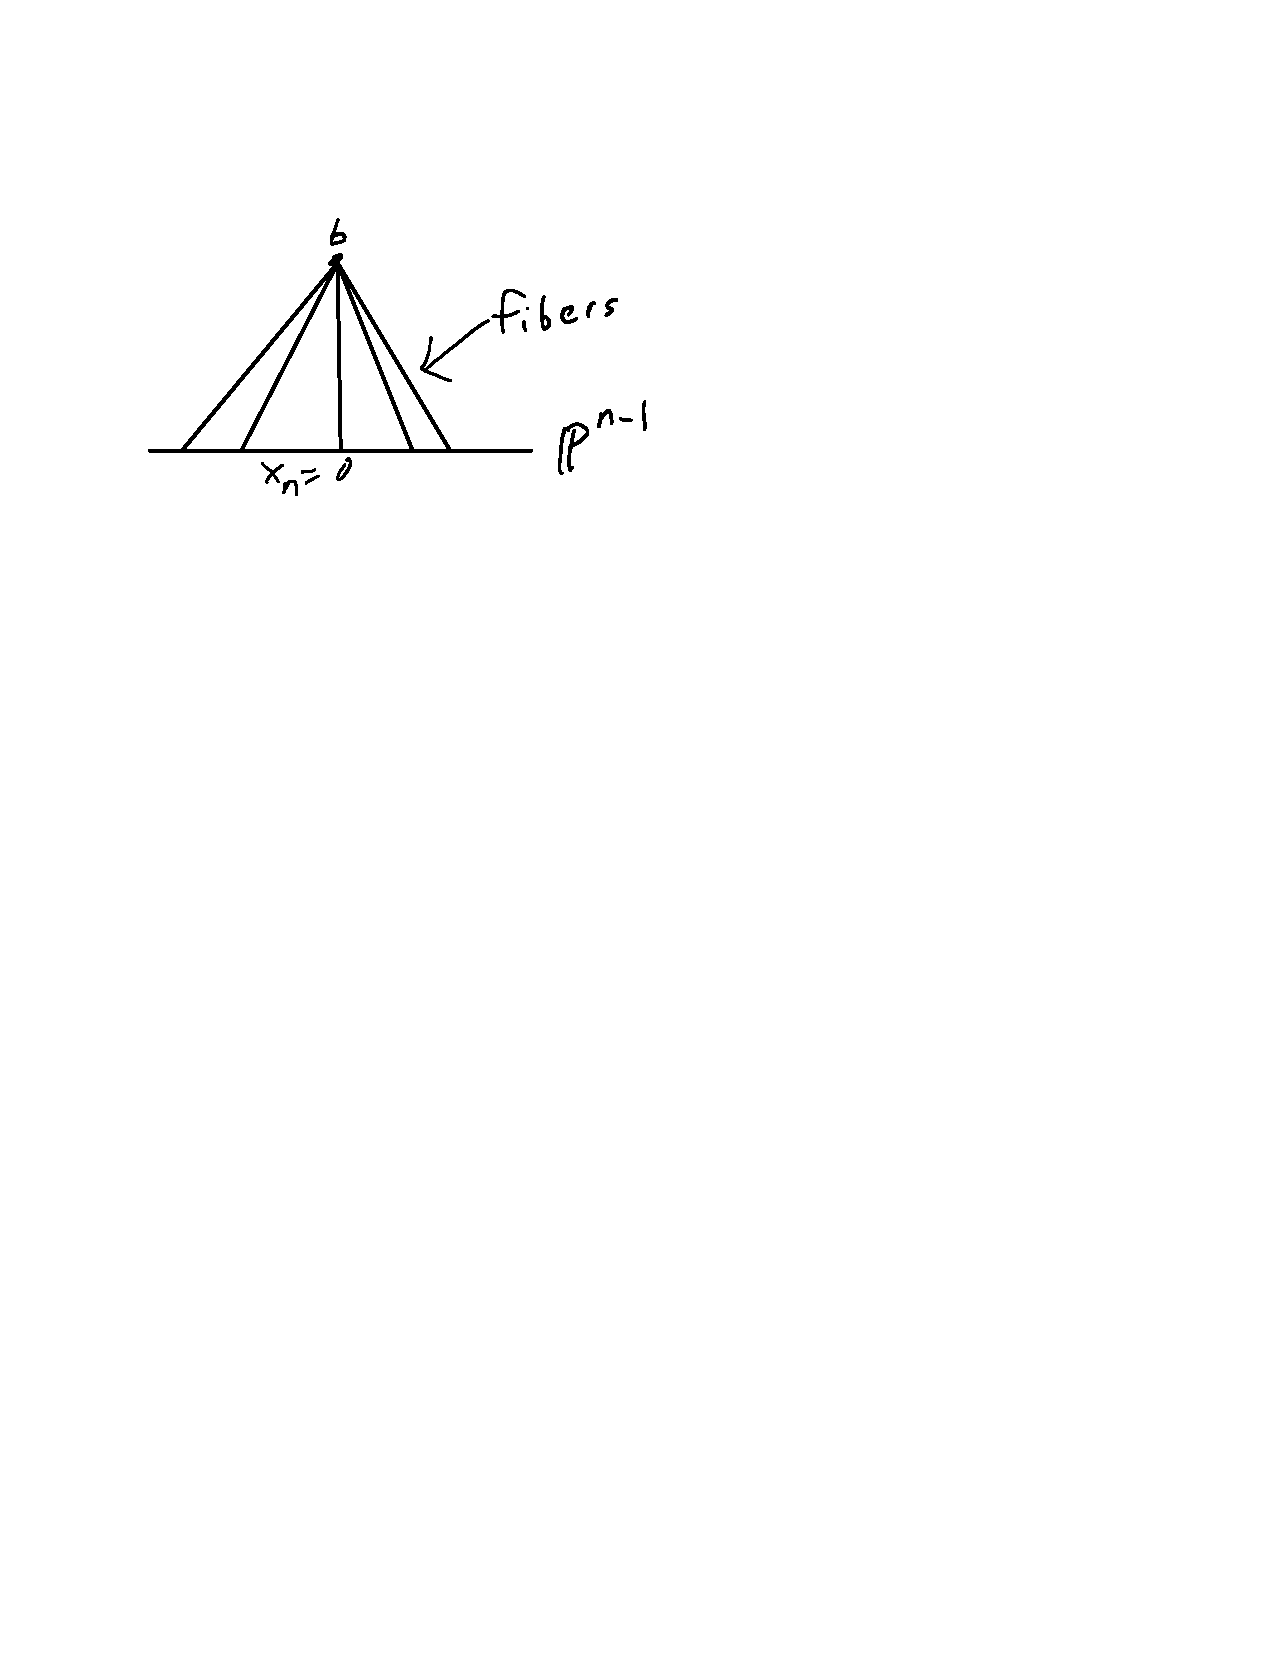
\includegraphics[width=0.5\textwidth]{2011-04-01_Diagram_001}\end{center}
  In $\mathbb P^n \times P^{n-1}$ let $\Gamma$ be the graph.  $\bar \Gamma$ is the Zariski closure of $\Gamma$.  Label the points $(x_i), (y_i) \in \mathbb P^n \times \mathbb P^{n-1}$.  $\Gamma$: $x_i = y_i$ for $i = 0, \ldots, n-1$.  The equations $x_i y_j - x_j y_i$ for $i, j = 0, \ldots, n-1$ define a Zariski closed set of $\bar \Gamma$.  Look where $x_0 \ne 0$: Take $x_0 = 1$.  Then $y_j = x_j y_0$.  We can't have $y_0 = 0$: Take $y_0 = 1$.  Then $y_j = x_j$, $j = 0, \ldots, n-1$, $x_n$ arbitrary.  Only the center $p = (0, 0, \ldots, 0, 1)$ escapes.  In this case, all the equations are trivial.  So no conditions on $(y)$.  The result is 
  $$\bar \Gamma = \mathset[(x, \pi(x))]{x\ne p} \cup \mathset[(p, y)]{y\text{ arbitrary}}.$$
  
  \emph{Grassmannians}: $G(r, n)$ is the $r$-dimensional subspace of $\mathbb C^n$.  For example, $\mathbb P^n = G(1, n+1)$.  Look at $G(2, 4) = 2$-dimensional subspaces of $\mathbb C^4$ or lines in $\mathbb P^3$.
  
  $V$ a vector space of dimension 4, basis $(v_1, v_2, v_3, v_4)$.  There is an exterior algebra $\bigwedge V$.  The rule is $vw = -wv$.  (Or $v\wedge w = -w\wedge v$.)  Then $vv = 0$.
  
  \noindent $\bigwedge^2 V$ has a basis $v_iv_j$ for $i = j$ dimension $\binom42 = 6$\\
  \noindent $\bigwedge^3 V$ has a basis $v_iv_jv_k$ for $i < j < k$ dimension 4 \\
  \noindent $\bigwedge^4 V$ has a basis $v_1v_2v_3v_4$  dimension 1 \\
  \noindent $\bigwedge^k V = 0$ for $k > 4$
  
  \begin{prop*} The following are equivalent:
    \begin{itemize}
      \item There is a subspace $W\subset V$ of dimension 2
      \item Vectors $w$ in $\bigwedge^2 V$, non-zero, and decomposable into $w = uv$, $u, v\in V$.
      \item $w$ in $\bigwedge^2 V$, $ww = 0$ $\big/ (\text{scalar})$
      \item Let $w = \sum\limits_{i<j} a_{ij}v_iv_j \longleftrightarrow (a_{ij})$ in $\mathbb P^5$.  Then $a_{12}a_{34} - a_{13}a_{24} + a_{14}a_{23} = 0$.
    \end{itemize}
  \end{prop*}
  \begin{proof}
    Partial sketch of one of the implications: $w = \sum a_{ij} u_i v_j$, $ww = \sum\limits_{i<j,k<l} a_{ij}a_{kl}v_iv_jv_kv_l$.  Plug in all the possible values.
  \end{proof}
\end{notessection}










\begin{notessection}{4}{4}{2011}
  
\end{notessection}


\end{document}